


% Header, overrides base

    % Make sure that the sphinx doc style knows who it inherits from.
    \def\sphinxdocclass{article}

    % Declare the document class
    \documentclass[letterpaper,10pt,english]{/usr/local/lib/python2.7/dist-packages/sphinx/texinputs/sphinxhowto}

    % Imports
    \usepackage[utf8]{inputenc}
    \DeclareUnicodeCharacter{00A0}{\\nobreakspace}
    \usepackage[T1]{fontenc}
    \usepackage{babel}
    \usepackage{times}
    \usepackage{import}
    \usepackage[Bjarne]{/usr/local/lib/python2.7/dist-packages/sphinx/texinputs/fncychap}
    \usepackage{longtable}
    \usepackage{/usr/local/lib/python2.7/dist-packages/sphinx/texinputs/sphinx}
    \usepackage{multirow}

    \usepackage{amsmath}
    \usepackage{amssymb}
    \usepackage{ucs}
    \usepackage{enumerate}

    % Used to make the Input/Output rules follow around the contents.
    \usepackage{needspace}

    % Pygments requirements
    \usepackage{fancyvrb}
    \usepackage{color}
    % ansi colors additions
    \definecolor{darkgreen}{rgb}{.12,.54,.11}
    \definecolor{lightgray}{gray}{.95}
    \definecolor{brown}{rgb}{0.54,0.27,0.07}
    \definecolor{purple}{rgb}{0.5,0.0,0.5}
    \definecolor{darkgray}{gray}{0.25}
    \definecolor{lightred}{rgb}{1.0,0.39,0.28}
    \definecolor{lightgreen}{rgb}{0.48,0.99,0.0}
    \definecolor{lightblue}{rgb}{0.53,0.81,0.92}
    \definecolor{lightpurple}{rgb}{0.87,0.63,0.87}
    \definecolor{lightcyan}{rgb}{0.5,1.0,0.83}

    % Needed to box output/input
    \usepackage{tikz}
        \usetikzlibrary{calc,arrows,shadows}
    \usepackage[framemethod=tikz]{mdframed}

    \usepackage{alltt}

    % Used to load and display graphics
    \usepackage{graphicx}
    \graphicspath{ {figs/} }
    \usepackage[Export]{adjustbox} % To resize

    % used so that images for notebooks which have spaces in the name can still be included
    \usepackage{grffile}


    % For formatting output while also word wrapping.
    \usepackage{listings}
    \lstset{breaklines=true}
    \lstset{basicstyle=\small\ttfamily}
    \def\smaller{\fontsize{9.5pt}{9.5pt}\selectfont}

    %Pygments definitions
    
\makeatletter
\def\PY@reset{\let\PY@it=\relax \let\PY@bf=\relax%
    \let\PY@ul=\relax \let\PY@tc=\relax%
    \let\PY@bc=\relax \let\PY@ff=\relax}
\def\PY@tok#1{\csname PY@tok@#1\endcsname}
\def\PY@toks#1+{\ifx\relax#1\empty\else%
    \PY@tok{#1}\expandafter\PY@toks\fi}
\def\PY@do#1{\PY@bc{\PY@tc{\PY@ul{%
    \PY@it{\PY@bf{\PY@ff{#1}}}}}}}
\def\PY#1#2{\PY@reset\PY@toks#1+\relax+\PY@do{#2}}

\expandafter\def\csname PY@tok@gd\endcsname{\def\PY@tc##1{\textcolor[rgb]{0.63,0.00,0.00}{##1}}}
\expandafter\def\csname PY@tok@gu\endcsname{\let\PY@bf=\textbf\def\PY@tc##1{\textcolor[rgb]{0.50,0.00,0.50}{##1}}}
\expandafter\def\csname PY@tok@gt\endcsname{\def\PY@tc##1{\textcolor[rgb]{0.00,0.27,0.87}{##1}}}
\expandafter\def\csname PY@tok@gs\endcsname{\let\PY@bf=\textbf}
\expandafter\def\csname PY@tok@gr\endcsname{\def\PY@tc##1{\textcolor[rgb]{1.00,0.00,0.00}{##1}}}
\expandafter\def\csname PY@tok@cm\endcsname{\let\PY@it=\textit\def\PY@tc##1{\textcolor[rgb]{0.25,0.50,0.50}{##1}}}
\expandafter\def\csname PY@tok@vg\endcsname{\def\PY@tc##1{\textcolor[rgb]{0.10,0.09,0.49}{##1}}}
\expandafter\def\csname PY@tok@m\endcsname{\def\PY@tc##1{\textcolor[rgb]{0.40,0.40,0.40}{##1}}}
\expandafter\def\csname PY@tok@mh\endcsname{\def\PY@tc##1{\textcolor[rgb]{0.40,0.40,0.40}{##1}}}
\expandafter\def\csname PY@tok@go\endcsname{\def\PY@tc##1{\textcolor[rgb]{0.53,0.53,0.53}{##1}}}
\expandafter\def\csname PY@tok@ge\endcsname{\let\PY@it=\textit}
\expandafter\def\csname PY@tok@vc\endcsname{\def\PY@tc##1{\textcolor[rgb]{0.10,0.09,0.49}{##1}}}
\expandafter\def\csname PY@tok@il\endcsname{\def\PY@tc##1{\textcolor[rgb]{0.40,0.40,0.40}{##1}}}
\expandafter\def\csname PY@tok@cs\endcsname{\let\PY@it=\textit\def\PY@tc##1{\textcolor[rgb]{0.25,0.50,0.50}{##1}}}
\expandafter\def\csname PY@tok@cp\endcsname{\def\PY@tc##1{\textcolor[rgb]{0.74,0.48,0.00}{##1}}}
\expandafter\def\csname PY@tok@gi\endcsname{\def\PY@tc##1{\textcolor[rgb]{0.00,0.63,0.00}{##1}}}
\expandafter\def\csname PY@tok@gh\endcsname{\let\PY@bf=\textbf\def\PY@tc##1{\textcolor[rgb]{0.00,0.00,0.50}{##1}}}
\expandafter\def\csname PY@tok@ni\endcsname{\let\PY@bf=\textbf\def\PY@tc##1{\textcolor[rgb]{0.60,0.60,0.60}{##1}}}
\expandafter\def\csname PY@tok@nl\endcsname{\def\PY@tc##1{\textcolor[rgb]{0.63,0.63,0.00}{##1}}}
\expandafter\def\csname PY@tok@nn\endcsname{\let\PY@bf=\textbf\def\PY@tc##1{\textcolor[rgb]{0.00,0.00,1.00}{##1}}}
\expandafter\def\csname PY@tok@no\endcsname{\def\PY@tc##1{\textcolor[rgb]{0.53,0.00,0.00}{##1}}}
\expandafter\def\csname PY@tok@na\endcsname{\def\PY@tc##1{\textcolor[rgb]{0.49,0.56,0.16}{##1}}}
\expandafter\def\csname PY@tok@nb\endcsname{\def\PY@tc##1{\textcolor[rgb]{0.00,0.50,0.00}{##1}}}
\expandafter\def\csname PY@tok@nc\endcsname{\let\PY@bf=\textbf\def\PY@tc##1{\textcolor[rgb]{0.00,0.00,1.00}{##1}}}
\expandafter\def\csname PY@tok@nd\endcsname{\def\PY@tc##1{\textcolor[rgb]{0.67,0.13,1.00}{##1}}}
\expandafter\def\csname PY@tok@ne\endcsname{\let\PY@bf=\textbf\def\PY@tc##1{\textcolor[rgb]{0.82,0.25,0.23}{##1}}}
\expandafter\def\csname PY@tok@nf\endcsname{\def\PY@tc##1{\textcolor[rgb]{0.00,0.00,1.00}{##1}}}
\expandafter\def\csname PY@tok@si\endcsname{\let\PY@bf=\textbf\def\PY@tc##1{\textcolor[rgb]{0.73,0.40,0.53}{##1}}}
\expandafter\def\csname PY@tok@s2\endcsname{\def\PY@tc##1{\textcolor[rgb]{0.73,0.13,0.13}{##1}}}
\expandafter\def\csname PY@tok@vi\endcsname{\def\PY@tc##1{\textcolor[rgb]{0.10,0.09,0.49}{##1}}}
\expandafter\def\csname PY@tok@nt\endcsname{\let\PY@bf=\textbf\def\PY@tc##1{\textcolor[rgb]{0.00,0.50,0.00}{##1}}}
\expandafter\def\csname PY@tok@nv\endcsname{\def\PY@tc##1{\textcolor[rgb]{0.10,0.09,0.49}{##1}}}
\expandafter\def\csname PY@tok@s1\endcsname{\def\PY@tc##1{\textcolor[rgb]{0.73,0.13,0.13}{##1}}}
\expandafter\def\csname PY@tok@kd\endcsname{\let\PY@bf=\textbf\def\PY@tc##1{\textcolor[rgb]{0.00,0.50,0.00}{##1}}}
\expandafter\def\csname PY@tok@sh\endcsname{\def\PY@tc##1{\textcolor[rgb]{0.73,0.13,0.13}{##1}}}
\expandafter\def\csname PY@tok@sc\endcsname{\def\PY@tc##1{\textcolor[rgb]{0.73,0.13,0.13}{##1}}}
\expandafter\def\csname PY@tok@sx\endcsname{\def\PY@tc##1{\textcolor[rgb]{0.00,0.50,0.00}{##1}}}
\expandafter\def\csname PY@tok@bp\endcsname{\def\PY@tc##1{\textcolor[rgb]{0.00,0.50,0.00}{##1}}}
\expandafter\def\csname PY@tok@c1\endcsname{\let\PY@it=\textit\def\PY@tc##1{\textcolor[rgb]{0.25,0.50,0.50}{##1}}}
\expandafter\def\csname PY@tok@kc\endcsname{\let\PY@bf=\textbf\def\PY@tc##1{\textcolor[rgb]{0.00,0.50,0.00}{##1}}}
\expandafter\def\csname PY@tok@c\endcsname{\let\PY@it=\textit\def\PY@tc##1{\textcolor[rgb]{0.25,0.50,0.50}{##1}}}
\expandafter\def\csname PY@tok@mf\endcsname{\def\PY@tc##1{\textcolor[rgb]{0.40,0.40,0.40}{##1}}}
\expandafter\def\csname PY@tok@err\endcsname{\def\PY@bc##1{\setlength{\fboxsep}{0pt}\fcolorbox[rgb]{1.00,0.00,0.00}{1,1,1}{\strut ##1}}}
\expandafter\def\csname PY@tok@mb\endcsname{\def\PY@tc##1{\textcolor[rgb]{0.40,0.40,0.40}{##1}}}
\expandafter\def\csname PY@tok@ss\endcsname{\def\PY@tc##1{\textcolor[rgb]{0.10,0.09,0.49}{##1}}}
\expandafter\def\csname PY@tok@sr\endcsname{\def\PY@tc##1{\textcolor[rgb]{0.73,0.40,0.53}{##1}}}
\expandafter\def\csname PY@tok@mo\endcsname{\def\PY@tc##1{\textcolor[rgb]{0.40,0.40,0.40}{##1}}}
\expandafter\def\csname PY@tok@kn\endcsname{\let\PY@bf=\textbf\def\PY@tc##1{\textcolor[rgb]{0.00,0.50,0.00}{##1}}}
\expandafter\def\csname PY@tok@mi\endcsname{\def\PY@tc##1{\textcolor[rgb]{0.40,0.40,0.40}{##1}}}
\expandafter\def\csname PY@tok@gp\endcsname{\let\PY@bf=\textbf\def\PY@tc##1{\textcolor[rgb]{0.00,0.00,0.50}{##1}}}
\expandafter\def\csname PY@tok@o\endcsname{\def\PY@tc##1{\textcolor[rgb]{0.40,0.40,0.40}{##1}}}
\expandafter\def\csname PY@tok@kr\endcsname{\let\PY@bf=\textbf\def\PY@tc##1{\textcolor[rgb]{0.00,0.50,0.00}{##1}}}
\expandafter\def\csname PY@tok@s\endcsname{\def\PY@tc##1{\textcolor[rgb]{0.73,0.13,0.13}{##1}}}
\expandafter\def\csname PY@tok@kp\endcsname{\def\PY@tc##1{\textcolor[rgb]{0.00,0.50,0.00}{##1}}}
\expandafter\def\csname PY@tok@w\endcsname{\def\PY@tc##1{\textcolor[rgb]{0.73,0.73,0.73}{##1}}}
\expandafter\def\csname PY@tok@kt\endcsname{\def\PY@tc##1{\textcolor[rgb]{0.69,0.00,0.25}{##1}}}
\expandafter\def\csname PY@tok@ow\endcsname{\let\PY@bf=\textbf\def\PY@tc##1{\textcolor[rgb]{0.67,0.13,1.00}{##1}}}
\expandafter\def\csname PY@tok@sb\endcsname{\def\PY@tc##1{\textcolor[rgb]{0.73,0.13,0.13}{##1}}}
\expandafter\def\csname PY@tok@k\endcsname{\let\PY@bf=\textbf\def\PY@tc##1{\textcolor[rgb]{0.00,0.50,0.00}{##1}}}
\expandafter\def\csname PY@tok@se\endcsname{\let\PY@bf=\textbf\def\PY@tc##1{\textcolor[rgb]{0.73,0.40,0.13}{##1}}}
\expandafter\def\csname PY@tok@sd\endcsname{\let\PY@it=\textit\def\PY@tc##1{\textcolor[rgb]{0.73,0.13,0.13}{##1}}}

\def\PYZbs{\char`\\}
\def\PYZus{\char`\_}
\def\PYZob{\char`\{}
\def\PYZcb{\char`\}}
\def\PYZca{\char`\^}
\def\PYZam{\char`\&}
\def\PYZlt{\char`\<}
\def\PYZgt{\char`\>}
\def\PYZsh{\char`\#}
\def\PYZpc{\char`\%}
\def\PYZdl{\char`\$}
\def\PYZhy{\char`\-}
\def\PYZsq{\char`\'}
\def\PYZdq{\char`\"}
\def\PYZti{\char`\~}
% for compatibility with earlier versions
\def\PYZat{@}
\def\PYZlb{[}
\def\PYZrb{]}
\makeatother


    %Set pygments styles if needed...
    
        \definecolor{nbframe-border}{rgb}{0.867,0.867,0.867}
        \definecolor{nbframe-bg}{rgb}{0.969,0.969,0.969}
        \definecolor{nbframe-in-prompt}{rgb}{0.0,0.0,0.502}
        \definecolor{nbframe-out-prompt}{rgb}{0.545,0.0,0.0}

        \newenvironment{ColorVerbatim}
        {\begin{mdframed}[%
            roundcorner=1.0pt, %
            backgroundcolor=nbframe-bg, %
            userdefinedwidth=1\linewidth, %
            leftmargin=0.1\linewidth, %
            innerleftmargin=0pt, %
            innerrightmargin=0pt, %
            linecolor=nbframe-border, %
            linewidth=1pt, %
            usetwoside=false, %
            everyline=true, %
            innerlinewidth=3pt, %
            innerlinecolor=nbframe-bg, %
            middlelinewidth=1pt, %
            middlelinecolor=nbframe-bg, %
            outerlinewidth=0.5pt, %
            outerlinecolor=nbframe-border, %
            needspace=0pt
        ]}
        {\end{mdframed}}
        
        \newenvironment{InvisibleVerbatim}
        {\begin{mdframed}[leftmargin=0.1\linewidth,innerleftmargin=3pt,innerrightmargin=3pt, userdefinedwidth=1\linewidth, linewidth=0pt, linecolor=white, usetwoside=false]}
        {\end{mdframed}}

        \renewenvironment{Verbatim}[1][\unskip]
        {\begin{alltt}\smaller}
        {\end{alltt}}
    

    % Help prevent overflowing lines due to urls and other hard-to-break 
    % entities.  This doesn't catch everything...
    \sloppy

    % Document level variables
    \title{Data\_Science\_HW\_1}
    \date{September 26, 2015}
    \release{}
    \author{Unknown Author}
    \renewcommand{\releasename}{}

    % TODO: Add option for the user to specify a logo for his/her export.
    \newcommand{\sphinxlogo}{}

    % Make the index page of the document.
    \makeindex

    % Import sphinx document type specifics.
     


% Body

    % Start of the document
    \begin{document}

        
            \maketitle
        

        


        
        

    % Make sure that atleast 4 lines are below the HR
    \needspace{4\baselineskip}

    
        \vspace{6pt}
        \makebox[0.1\linewidth]{\smaller\hfill\tt\color{nbframe-in-prompt}In\hspace{4pt}{[}1{]}:\hspace{4pt}}\\*
        \vspace{-2.65\baselineskip}
        \begin{ColorVerbatim}
            \vspace{-0.7\baselineskip}
            \begin{Verbatim}[commandchars=\\\{\}]
\PY{o}{\PYZpc{}}\PY{k}{matplotlib} \PY{n}{inline}

\PY{k+kn}{import} \PY{n+nn}{matplotlib} 
\PY{k+kn}{import} \PY{n+nn}{csv}
\PY{k+kn}{import} \PY{n+nn}{numpy} \PY{k+kn}{as} \PY{n+nn}{np}
\PY{k+kn}{import} \PY{n+nn}{matplotlib.pyplot} \PY{k+kn}{as} \PY{n+nn}{plt}
\PY{k+kn}{from} \PY{n+nn}{scipy} \PY{k+kn}{import} \PY{n}{stats}
\end{Verbatim}

            
                \vspace{-0.2\baselineskip}
            
        \end{ColorVerbatim}
    
Here we define some utility functions used in parsing and cleaning the
data.

    % Make sure that atleast 4 lines are below the HR
    \needspace{4\baselineskip}

    
        \vspace{6pt}
        \makebox[0.1\linewidth]{\smaller\hfill\tt\color{nbframe-in-prompt}In\hspace{4pt}{[}2{]}:\hspace{4pt}}\\*
        \vspace{-2.65\baselineskip}
        \begin{ColorVerbatim}
            \vspace{-0.7\baselineskip}
            \begin{Verbatim}[commandchars=\\\{\}]
\PY{k}{def} \PY{n+nf}{isnum}\PY{p}{(}\PY{n}{a}\PY{p}{)}\PY{p}{:}
    \PY{k}{try}\PY{p}{:}
        \PY{n+nb}{float}\PY{p}{(}\PY{n}{a}\PY{p}{)}
    \PY{k}{except} \PY{n+ne}{ValueError}\PY{p}{:}
        \PY{k}{return} \PY{n+nb+bp}{False}
    \PY{k}{return} \PY{n+nb+bp}{True}
\PY{k}{def} \PY{n+nf}{reject\PYZus{}outliers}\PY{p}{(}\PY{n}{data}\PY{p}{,} \PY{n}{m}\PY{o}{=}\PY{l+m+mi}{2}\PY{p}{)}\PY{p}{:}
    \PY{k}{return} \PY{n}{data}\PY{p}{[}\PY{n}{np}\PY{o}{.}\PY{n}{logical\PYZus{}and}\PY{p}{(}\PY{n+nb}{abs}\PY{p}{(}\PY{n}{data} \PY{o}{\PYZhy{}} \PY{n}{np}\PY{o}{.}\PY{n}{mean}\PY{p}{(}\PY{n}{data}\PY{p}{)}\PY{p}{)} \PY{o}{\PYZlt{}} \PY{n}{m} \PY{o}{*} \PY{n}{np}\PY{o}{.}\PY{n}{std}\PY{p}{(}\PY{n}{data}\PY{p}{)}\PY{p}{,}\PY{n}{data} \PY{o}{\PYZgt{}} \PY{l+m+mi}{0}\PY{p}{)}\PY{p}{]}
\PY{k}{def} \PY{n+nf}{get\PYZus{}stats}\PY{p}{(}\PY{n}{data}\PY{p}{,} \PY{n}{index}\PY{p}{)}\PY{p}{:}
    \PY{n}{overall} \PY{o}{=} \PY{n}{np}\PY{o}{.}\PY{n}{array}\PY{p}{(}\PY{p}{[}\PY{n}{x} \PY{k}{for} \PY{n}{x} \PY{o+ow}{in} \PY{n}{data}\PY{p}{[}\PY{l+m+mi}{1}\PY{p}{:}\PY{p}{,}\PY{n}{index}\PY{p}{]} \PY{k}{if} \PY{n}{isnum}\PY{p}{(}\PY{n}{x}\PY{p}{)}\PY{p}{]}\PY{p}{)}\PY{o}{.}\PY{n}{astype}\PY{p}{(}\PY{n}{np}\PY{o}{.}\PY{n}{float}\PY{p}{)}
    \PY{n}{overall} \PY{o}{=} \PY{n}{reject\PYZus{}outliers}\PY{p}{(}\PY{n}{overall}\PY{p}{,}\PY{l+m+mi}{2}\PY{p}{)}
    \PY{n}{overallStats} \PY{o}{=} \PY{p}{(}\PY{n}{np}\PY{o}{.}\PY{n}{mean}\PY{p}{(}\PY{n}{overall}\PY{p}{)}\PY{p}{,} \PY{n}{np}\PY{o}{.}\PY{n}{median}\PY{p}{(}\PY{n}{overall}\PY{p}{)}\PY{p}{,} \PY{n}{stats}\PY{o}{.}\PY{n}{mode}\PY{p}{(}\PY{n}{overall}\PY{p}{)}\PY{p}{,} \PY{n}{np}\PY{o}{.}\PY{n}{std}\PY{p}{(}\PY{n}{overall}\PY{p}{)}\PY{p}{,} \PY{n}{np}\PY{o}{.}\PY{n}{max}\PY{p}{(}\PY{n}{overall}\PY{p}{)}\PY{p}{,} \PY{n}{np}\PY{o}{.}\PY{n}{min}\PY{p}{(}\PY{n}{overall}\PY{p}{)}\PY{p}{)}
    \PY{k}{return} \PY{n}{overall}\PY{p}{,} \PY{n}{overallStats}
\end{Verbatim}

            
                \vspace{-0.2\baselineskip}
            
        \end{ColorVerbatim}
    


    % Make sure that atleast 4 lines are below the HR
    \needspace{4\baselineskip}

    
        \vspace{6pt}
        \makebox[0.1\linewidth]{\smaller\hfill\tt\color{nbframe-in-prompt}In\hspace{4pt}{[}3{]}:\hspace{4pt}}\\*
        \vspace{-2.65\baselineskip}
        \begin{ColorVerbatim}
            \vspace{-0.7\baselineskip}
            \begin{Verbatim}[commandchars=\\\{\}]
\PY{n}{movies} \PY{o}{=} \PY{p}{[}\PY{p}{]}
\PY{k}{with} \PY{n+nb}{open}\PY{p}{(}\PY{l+s}{\PYZsq{}}\PY{l+s}{movies.csv}\PY{l+s}{\PYZsq{}}\PY{p}{,} \PY{l+s}{\PYZsq{}}\PY{l+s}{rb}\PY{l+s}{\PYZsq{}}\PY{p}{)} \PY{k}{as} \PY{n}{csvfile}\PY{p}{:}
    \PY{n}{moviereader} \PY{o}{=} \PY{n}{csv}\PY{o}{.}\PY{n}{reader}\PY{p}{(}\PY{n}{csvfile}\PY{p}{)}
    \PY{k}{for} \PY{n}{row} \PY{o+ow}{in} \PY{n}{moviereader}\PY{p}{:}
        \PY{n}{movies}\PY{o}{.}\PY{n}{append}\PY{p}{(}\PY{n}{row}\PY{p}{)}
\PY{n}{movies} \PY{o}{=} \PY{n}{np}\PY{o}{.}\PY{n}{array}\PY{p}{(}\PY{n}{movies}\PY{p}{)}
\end{Verbatim}

            
                \vspace{-0.2\baselineskip}
            
        \end{ColorVerbatim}
    
\section{Problem 1 - Worldwide Distribution}Now we calculate some central tendency measures for all movies' gross
and plot a box plot!

When cleaning the data, some movies have the value ``Unknown'' for their
gross, which is not convertible to a float. That's why we take only
values that return true for isnum().

The data is heavily centered at low gross profits, with an exponential
tail towards very high profits. Honestly I'm not sure how to deal with a
set of data that is so heavily skewed. I reject outliers that are more
than 2 standard deviations from the mean as it's a commonly used method
and I'm no statistician.

The mode isn't particularly helpful. The median is significantly below
the mean for this data, implying there are a few movies that do
exceptionally well while most have low grosses.

    % Make sure that atleast 4 lines are below the HR
    \needspace{4\baselineskip}

    
        \vspace{6pt}
        \makebox[0.1\linewidth]{\smaller\hfill\tt\color{nbframe-in-prompt}In\hspace{4pt}{[}4{]}:\hspace{4pt}}\\*
        \vspace{-2.65\baselineskip}
        \begin{ColorVerbatim}
            \vspace{-0.7\baselineskip}
            \begin{Verbatim}[commandchars=\\\{\}]
\PY{n}{wwgross\PYZus{}pre} \PY{o}{=} \PY{n}{np}\PY{o}{.}\PY{n}{array}\PY{p}{(}\PY{p}{[}\PY{n}{x} \PY{k}{for} \PY{n}{x} \PY{o+ow}{in} \PY{n}{movies}\PY{p}{[}\PY{l+m+mi}{1}\PY{p}{:}\PY{p}{,}\PY{l+m+mi}{2}\PY{p}{]} \PY{k}{if} \PY{n}{isnum}\PY{p}{(}\PY{n}{x}\PY{p}{)}\PY{p}{]}\PY{p}{)}\PY{o}{.}\PY{n}{astype}\PY{p}{(}\PY{n}{np}\PY{o}{.}\PY{n}{float}\PY{p}{)}
\PY{n}{wwgross} \PY{o}{=} \PY{n}{reject\PYZus{}outliers}\PY{p}{(}\PY{n}{wwgross\PYZus{}pre}\PY{p}{,}\PY{l+m+mi}{2}\PY{p}{)}
\PY{n}{wwGrossStats} \PY{o}{=} \PY{p}{(}\PY{n}{np}\PY{o}{.}\PY{n}{mean}\PY{p}{(}\PY{n}{wwgross}\PY{p}{)}\PY{p}{,} \PY{n}{np}\PY{o}{.}\PY{n}{median}\PY{p}{(}\PY{n}{wwgross}\PY{p}{)}\PY{p}{,} \PY{n}{stats}\PY{o}{.}\PY{n}{mode}\PY{p}{(}\PY{n}{wwgross}\PY{p}{)}\PY{p}{,} \PY{n}{np}\PY{o}{.}\PY{n}{std}\PY{p}{(}\PY{n}{wwgross}\PY{p}{)}\PY{p}{,} \PY{n}{np}\PY{o}{.}\PY{n}{max}\PY{p}{(}\PY{n}{wwgross}\PY{p}{)}\PY{p}{,} \PY{n}{np}\PY{o}{.}\PY{n}{min}\PY{p}{(}\PY{n}{wwgross}\PY{p}{)}\PY{p}{)}
\PY{k}{print} \PY{n}{wwGrossStats}
\end{Verbatim}

            
                \vspace{-0.2\baselineskip}
            
        \end{ColorVerbatim}
    

    

        % If the first block is an image, minipage the image.  Else
        % request a certain amount of space for the input text.
        \needspace{4\baselineskip}
        
        

            % Add document contents.
            
                \begin{InvisibleVerbatim}
                \vspace{-0.5\baselineskip}
\begin{alltt}(63227637.950645909, 29367143.0, (array([ 8000000.]), array([ 9.])),
81725815.301398709, 385000317.0, 401.0)
\end{alltt}

            \end{InvisibleVerbatim}
            
        
    


    % Make sure that atleast 4 lines are below the HR
    \needspace{4\baselineskip}

    
        \vspace{6pt}
        \makebox[0.1\linewidth]{\smaller\hfill\tt\color{nbframe-in-prompt}In\hspace{4pt}{[}5{]}:\hspace{4pt}}\\*
        \vspace{-2.65\baselineskip}
        \begin{ColorVerbatim}
            \vspace{-0.7\baselineskip}
            \begin{Verbatim}[commandchars=\\\{\}]
\PY{n}{fig} \PY{o}{=} \PY{n}{plt}\PY{o}{.}\PY{n}{figure}\PY{p}{(}\PY{p}{)}
\PY{n}{ax} \PY{o}{=} \PY{n}{fig}\PY{o}{.}\PY{n}{add\PYZus{}subplot}\PY{p}{(}\PY{l+m+mi}{111}\PY{p}{)}
\PY{n}{ax}\PY{o}{.}\PY{n}{hist}\PY{p}{(}\PY{n}{wwgross\PYZus{}pre}\PY{p}{)}
\PY{n}{plt}\PY{o}{.}\PY{n}{show}\PY{p}{(}\PY{p}{)}

\PY{n}{fig} \PY{o}{=} \PY{n}{plt}\PY{o}{.}\PY{n}{figure}\PY{p}{(}\PY{p}{)}
\PY{n}{ax} \PY{o}{=} \PY{n}{fig}\PY{o}{.}\PY{n}{add\PYZus{}subplot}\PY{p}{(}\PY{l+m+mi}{111}\PY{p}{)}
\PY{n}{ax}\PY{o}{.}\PY{n}{hist}\PY{p}{(}\PY{n}{wwgross}\PY{p}{)}
\PY{n}{plt}\PY{o}{.}\PY{n}{show}\PY{p}{(}\PY{p}{)}
\end{Verbatim}

            
                \vspace{-0.2\baselineskip}
            
        \end{ColorVerbatim}
    

    

        % If the first block is an image, minipage the image.  Else
        % request a certain amount of space for the input text.
        \needspace{4\baselineskip}
        
        

            % Add document contents.
            
                \begin{InvisibleVerbatim}
                \vspace{-0.5\baselineskip}
    \begin{center}
    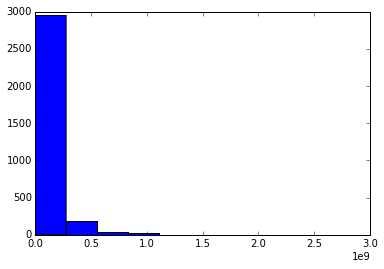
\includegraphics[max size={\textwidth}{\textheight}]{Data_Science_HW_1_files/Data_Science_HW_1_7_0.png}
    \par
    \end{center}
    
            \end{InvisibleVerbatim}
            
                \begin{InvisibleVerbatim}
                \vspace{-0.5\baselineskip}
    \begin{center}
    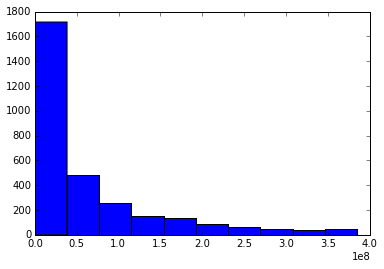
\includegraphics[max size={\textwidth}{\textheight}]{Data_Science_HW_1_files/Data_Science_HW_1_7_1.png}
    \par
    \end{center}
    
            \end{InvisibleVerbatim}
            
        
    


    % Make sure that atleast 4 lines are below the HR
    \needspace{4\baselineskip}

    
        \vspace{6pt}
        \makebox[0.1\linewidth]{\smaller\hfill\tt\color{nbframe-in-prompt}In\hspace{4pt}{[}6{]}:\hspace{4pt}}\\*
        \vspace{-2.65\baselineskip}
        \begin{ColorVerbatim}
            \vspace{-0.7\baselineskip}
            \begin{Verbatim}[commandchars=\\\{\}]
\PY{n}{fig} \PY{o}{=} \PY{n}{plt}\PY{o}{.}\PY{n}{figure}\PY{p}{(}\PY{p}{)}
\PY{n}{ax} \PY{o}{=} \PY{n}{fig}\PY{o}{.}\PY{n}{add\PYZus{}subplot}\PY{p}{(}\PY{l+m+mi}{111}\PY{p}{)}
\PY{n}{ax}\PY{o}{.}\PY{n}{boxplot}\PY{p}{(}\PY{n}{wwgross}\PY{p}{)}
\PY{n}{plt}\PY{o}{.}\PY{n}{show}\PY{p}{(}\PY{p}{)}
\end{Verbatim}

            
                \vspace{-0.2\baselineskip}
            
        \end{ColorVerbatim}
    

    

        % If the first block is an image, minipage the image.  Else
        % request a certain amount of space for the input text.
        \needspace{4\baselineskip}
        
        

            % Add document contents.
            
                \begin{InvisibleVerbatim}
                \vspace{-0.5\baselineskip}
    \begin{center}
    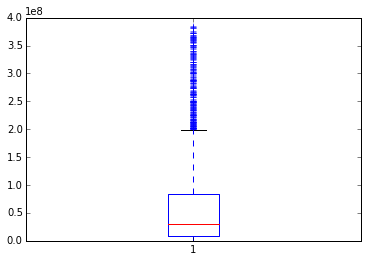
\includegraphics[max size={\textwidth}{\textheight}]{Data_Science_HW_1_files/Data_Science_HW_1_8_0.png}
    \par
    \end{center}
    
            \end{InvisibleVerbatim}
            
        
    
We now turn to analyzing the top-5 distributors of movies, following the
same process as above.

    % Make sure that atleast 4 lines are below the HR
    \needspace{4\baselineskip}

    
        \vspace{6pt}
        \makebox[0.1\linewidth]{\smaller\hfill\tt\color{nbframe-in-prompt}In\hspace{4pt}{[}7{]}:\hspace{4pt}}\\*
        \vspace{-2.65\baselineskip}
        \begin{ColorVerbatim}
            \vspace{-0.7\baselineskip}
            \begin{Verbatim}[commandchars=\\\{\}]
\PY{n}{distributors} \PY{o}{=} \PY{p}{[}\PY{p}{]}
\PY{n}{dist\PYZus{}i} \PY{o}{=} \PY{l+m+mi}{8}
\PY{k}{for} \PY{n}{row} \PY{o+ow}{in} \PY{n}{movies}\PY{p}{[}\PY{l+m+mi}{1}\PY{p}{:}\PY{p}{]}\PY{p}{:}
    \PY{k}{if} \PY{n}{row}\PY{p}{[}\PY{n}{dist\PYZus{}i}\PY{p}{]} \PY{o+ow}{not} \PY{o+ow}{in} \PY{n}{distributors}\PY{p}{:}
        \PY{n}{distributors}\PY{o}{.}\PY{n}{append}\PY{p}{(}\PY{n}{row}\PY{p}{[}\PY{n}{dist\PYZus{}i}\PY{p}{]}\PY{p}{)}
\end{Verbatim}

            
                \vspace{-0.2\baselineskip}
            
        \end{ColorVerbatim}
    


    % Make sure that atleast 4 lines are below the HR
    \needspace{4\baselineskip}

    
        \vspace{6pt}
        \makebox[0.1\linewidth]{\smaller\hfill\tt\color{nbframe-in-prompt}In\hspace{4pt}{[}8{]}:\hspace{4pt}}\\*
        \vspace{-2.65\baselineskip}
        \begin{ColorVerbatim}
            \vspace{-0.7\baselineskip}
            \begin{Verbatim}[commandchars=\\\{\}]
\PY{n}{dist\PYZus{}grouped} \PY{o}{=} \PY{p}{[}\PY{p}{]}
\PY{k}{for} \PY{n}{d} \PY{o+ow}{in} \PY{n}{distributors}\PY{p}{:}
    \PY{n}{dist\PYZus{}grouped}\PY{o}{.}\PY{n}{append}\PY{p}{(} \PY{p}{[}\PY{n}{d}\PY{p}{,} \PY{n}{np}\PY{o}{.}\PY{n}{array}\PY{p}{(}\PY{p}{[}\PY{n}{row} \PY{k}{for} \PY{n}{row} \PY{o+ow}{in} \PY{n}{movies} \PY{k}{if} \PY{n}{row}\PY{p}{[}\PY{n}{dist\PYZus{}i}\PY{p}{]} \PY{o}{==} \PY{n}{d}\PY{p}{]}\PY{p}{)}\PY{p}{]}\PY{p}{)}
\end{Verbatim}

            
                \vspace{-0.2\baselineskip}
            
        \end{ColorVerbatim}
    


    % Make sure that atleast 4 lines are below the HR
    \needspace{4\baselineskip}

    
        \vspace{6pt}
        \makebox[0.1\linewidth]{\smaller\hfill\tt\color{nbframe-in-prompt}In\hspace{4pt}{[}9{]}:\hspace{4pt}}\\*
        \vspace{-2.65\baselineskip}
        \begin{ColorVerbatim}
            \vspace{-0.7\baselineskip}
            \begin{Verbatim}[commandchars=\\\{\}]
\PY{n}{dist\PYZus{}sums} \PY{o}{=} \PY{p}{[}\PY{p}{]}
\PY{k}{for} \PY{n}{d} \PY{o+ow}{in} \PY{n}{dist\PYZus{}grouped}\PY{p}{:}
    \PY{n}{dist\PYZus{}sums}\PY{o}{.}\PY{n}{append}\PY{p}{(}\PY{p}{(}\PY{p}{[}\PY{n}{d}\PY{p}{[}\PY{l+m+mi}{0}\PY{p}{]}\PY{p}{,}\PY{n+nb}{sum}\PY{p}{(}\PY{n}{np}\PY{o}{.}\PY{n}{array}\PY{p}{(}\PY{p}{[}\PY{n}{x} \PY{k}{for} \PY{n}{x} \PY{o+ow}{in} \PY{n}{d}\PY{p}{[}\PY{l+m+mi}{1}\PY{p}{]}\PY{p}{[}\PY{p}{:}\PY{p}{,}\PY{l+m+mi}{2}\PY{p}{]} \PY{k}{if} \PY{n}{isnum}\PY{p}{(}\PY{n}{x}\PY{p}{)}\PY{p}{]}\PY{p}{)}\PY{o}{.}\PY{n}{astype}\PY{p}{(}\PY{n}{np}\PY{o}{.}\PY{n}{float}\PY{p}{)}\PY{p}{)}\PY{p}{]}\PY{p}{)}\PY{p}{)}
\PY{n}{dist\PYZus{}sums}\PY{o}{.}\PY{n}{sort}\PY{p}{(}\PY{n}{key}\PY{o}{=} \PY{k}{lambda} \PY{n}{x}\PY{p}{:} \PY{n}{x}\PY{p}{[}\PY{l+m+mi}{1}\PY{p}{]}\PY{p}{,} \PY{n}{reverse}\PY{o}{=}\PY{n+nb+bp}{True}\PY{p}{)}
\PY{n}{top6} \PY{o}{=} \PY{n}{dist\PYZus{}sums}\PY{p}{[}\PY{p}{:}\PY{l+m+mi}{6}\PY{p}{]}
\PY{k}{print} \PY{n}{top6}
\end{Verbatim}

            
                \vspace{-0.2\baselineskip}
            
        \end{ColorVerbatim}
    

    

        % If the first block is an image, minipage the image.  Else
        % request a certain amount of space for the input text.
        \needspace{4\baselineskip}
        
        

            % Add document contents.
            
                \begin{InvisibleVerbatim}
                \vspace{-0.5\baselineskip}
\begin{alltt}[['Warner Bros.', 39712039384.0], ['Walt Disney Pictures',
35458388004.0], ['20th Century Fox', 34739813057.0], ['Paramount
Pictures', 34361820057.0], ['Sony Pictures', 32418346390.0],
['Universal', 30356787647.0]]
\end{alltt}

            \end{InvisibleVerbatim}
            
        
    


    % Make sure that atleast 4 lines are below the HR
    \needspace{4\baselineskip}

    
        \vspace{6pt}
        \makebox[0.1\linewidth]{\smaller\hfill\tt\color{nbframe-in-prompt}In\hspace{4pt}{[}10{]}:\hspace{4pt}}\\*
        \vspace{-2.65\baselineskip}
        \begin{ColorVerbatim}
            \vspace{-0.7\baselineskip}
            \begin{Verbatim}[commandchars=\\\{\}]
\PY{n}{top6\PYZus{}rows} \PY{o}{=} \PY{p}{[}\PY{p}{]}
\PY{k}{for} \PY{n}{top} \PY{o+ow}{in} \PY{n}{top6}\PY{p}{:}
    \PY{n}{top6\PYZus{}rows}\PY{o}{.}\PY{n}{append}\PY{p}{(}\PY{p}{[}\PY{n}{top}\PY{p}{[}\PY{l+m+mi}{0}\PY{p}{]}\PY{p}{,} \PY{p}{[}\PY{n}{row} \PY{k}{for} \PY{n}{row} \PY{o+ow}{in} \PY{n}{movies} \PY{k}{if} \PY{n}{row}\PY{p}{[}\PY{n}{dist\PYZus{}i}\PY{p}{]} \PY{o}{==} \PY{n}{top}\PY{p}{[}\PY{l+m+mi}{0}\PY{p}{]}\PY{p}{]}\PY{p}{]}\PY{p}{)}
\end{Verbatim}

            
                \vspace{-0.2\baselineskip}
            
        \end{ColorVerbatim}
    


    % Make sure that atleast 4 lines are below the HR
    \needspace{4\baselineskip}

    
        \vspace{6pt}
        \makebox[0.1\linewidth]{\smaller\hfill\tt\color{nbframe-in-prompt}In\hspace{4pt}{[}11{]}:\hspace{4pt}}\\*
        \vspace{-2.65\baselineskip}
        \begin{ColorVerbatim}
            \vspace{-0.7\baselineskip}
            \begin{Verbatim}[commandchars=\\\{\}]
\PY{k}{for} \PY{n}{big\PYZus{}dist} \PY{o+ow}{in} \PY{n}{top6\PYZus{}rows}\PY{p}{:}
    \PY{n}{dist} \PY{o}{=} \PY{n}{np}\PY{o}{.}\PY{n}{array}\PY{p}{(}\PY{n}{big\PYZus{}dist}\PY{p}{[}\PY{l+m+mi}{1}\PY{p}{:}\PY{p}{]}\PY{p}{[}\PY{l+m+mi}{0}\PY{p}{]}\PY{p}{)}
    \PY{n}{wwgross} \PY{o}{=} \PY{n}{np}\PY{o}{.}\PY{n}{array}\PY{p}{(}\PY{p}{[}\PY{n}{x} \PY{k}{for} \PY{n}{x} \PY{o+ow}{in} \PY{n}{dist}\PY{p}{[}\PY{p}{:}\PY{p}{,}\PY{l+m+mi}{2}\PY{p}{]} \PY{k}{if} \PY{n}{isnum}\PY{p}{(}\PY{n}{x}\PY{p}{)}\PY{p}{]}\PY{p}{)}\PY{o}{.}\PY{n}{astype}\PY{p}{(}\PY{n}{np}\PY{o}{.}\PY{n}{float}\PY{p}{)}
    \PY{n}{wwgross} \PY{o}{=} \PY{n}{reject\PYZus{}outliers}\PY{p}{(}\PY{n}{wwgross}\PY{p}{,}\PY{l+m+mi}{2}\PY{p}{)}
    \PY{n}{wwGrossStats} \PY{o}{=} \PY{p}{(}\PY{n}{np}\PY{o}{.}\PY{n}{mean}\PY{p}{(}\PY{n}{wwgross}\PY{p}{)}\PY{p}{,} \PY{n}{np}\PY{o}{.}\PY{n}{median}\PY{p}{(}\PY{n}{wwgross}\PY{p}{)}\PY{p}{,} \PY{n}{stats}\PY{o}{.}\PY{n}{mode}\PY{p}{(}\PY{n}{wwgross}\PY{p}{)}\PY{p}{,} \PY{n}{np}\PY{o}{.}\PY{n}{std}\PY{p}{(}\PY{n}{wwgross}\PY{p}{)}\PY{p}{,} \PY{n}{np}\PY{o}{.}\PY{n}{min}\PY{p}{(}\PY{n}{wwgross}\PY{p}{)}\PY{p}{,} \PY{n}{np}\PY{o}{.}\PY{n}{max}\PY{p}{(}\PY{n}{wwgross}\PY{p}{)}\PY{p}{)}
    \PY{k}{print} \PY{l+s}{\PYZdq{}}\PY{l+s}{Mean : Median : Mode : Std : Min : Max}\PY{l+s}{\PYZdq{}}
    \PY{k}{print} \PY{n}{wwGrossStats}
    \PY{n}{fig} \PY{o}{=} \PY{n}{plt}\PY{o}{.}\PY{n}{figure}\PY{p}{(}\PY{p}{)}
    \PY{n}{ax} \PY{o}{=} \PY{n}{fig}\PY{o}{.}\PY{n}{add\PYZus{}subplot}\PY{p}{(}\PY{l+m+mi}{111}\PY{p}{)}
    \PY{n}{ax}\PY{o}{.}\PY{n}{boxplot}\PY{p}{(}\PY{n}{wwgross}\PY{p}{)}
    \PY{n}{plt}\PY{o}{.}\PY{n}{show}\PY{p}{(}\PY{p}{)}
\end{Verbatim}

            
                \vspace{-0.2\baselineskip}
            
        \end{ColorVerbatim}
    

    

        % If the first block is an image, minipage the image.  Else
        % request a certain amount of space for the input text.
        \needspace{4\baselineskip}
        
        

            % Add document contents.
            
                \begin{InvisibleVerbatim}
                \vspace{-0.5\baselineskip}
\begin{alltt}Mean : Median : Mode : Std : Min : Max
(97946257.976897687, 54540662.0, (array([ 5000000.]), array([ 2.])),
110985453.83315636, 126247.0, 474459076.0)
\end{alltt}

            \end{InvisibleVerbatim}
            
                \begin{InvisibleVerbatim}
                \vspace{-0.5\baselineskip}
    \begin{center}
    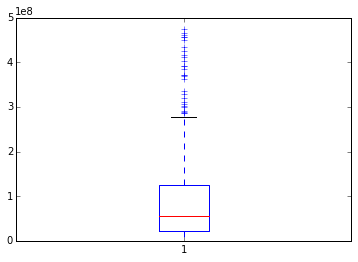
\includegraphics[max size={\textwidth}{\textheight}]{Data_Science_HW_1_files/Data_Science_HW_1_14_1.png}
    \par
    \end{center}
    
            \end{InvisibleVerbatim}
            
                \begin{InvisibleVerbatim}
                \vspace{-0.5\baselineskip}
\begin{alltt}Mean : Median : Mode : Std : Min : Max
(116586633.79545455, 66459170.5, (array([ 45779.]), array([ 1.])),
127689287.14854014, 45779.0, 554600000.0)
\end{alltt}

            \end{InvisibleVerbatim}
            
                \begin{InvisibleVerbatim}
                \vspace{-0.5\baselineskip}
    \begin{center}
    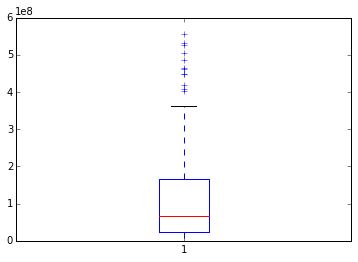
\includegraphics[max size={\textwidth}{\textheight}]{Data_Science_HW_1_files/Data_Science_HW_1_14_3.png}
    \par
    \end{center}
    
            \end{InvisibleVerbatim}
            
                \begin{InvisibleVerbatim}
                \vspace{-0.5\baselineskip}
\begin{alltt}Mean : Median : Mode : Std : Min : Max
(119945693.94545455, 62984793.5, (array([ 388390.]), array([ 1.])),
132172402.91969429, 388390.0, 574480841.0)
\end{alltt}

            \end{InvisibleVerbatim}
            
                \begin{InvisibleVerbatim}
                \vspace{-0.5\baselineskip}
    \begin{center}
    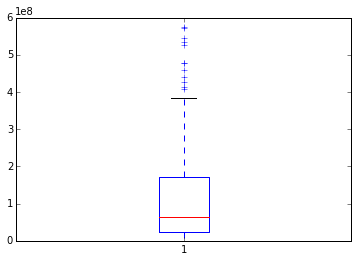
\includegraphics[max size={\textwidth}{\textheight}]{Data_Science_HW_1_files/Data_Science_HW_1_14_5.png}
    \par
    \end{center}
    
            \end{InvisibleVerbatim}
            
                \begin{InvisibleVerbatim}
                \vspace{-0.5\baselineskip}
\begin{alltt}Mean : Median : Mode : Std : Min : Max
(101323331.64876033, 64119833.0, (array([ 54606.]), array([ 1.])),
101067607.89296441, 54606.0, 491581231.0)
\end{alltt}

            \end{InvisibleVerbatim}
            
                \begin{InvisibleVerbatim}
                \vspace{-0.5\baselineskip}
    \begin{center}
    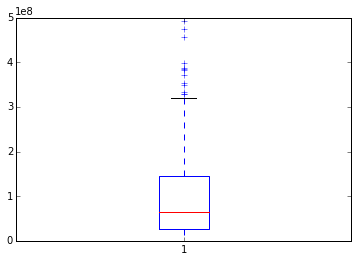
\includegraphics[max size={\textwidth}{\textheight}]{Data_Science_HW_1_files/Data_Science_HW_1_14_7.png}
    \par
    \end{center}
    
            \end{InvisibleVerbatim}
            
                \begin{InvisibleVerbatim}
                \vspace{-0.5\baselineskip}
\begin{alltt}Mean : Median : Mode : Std : Min : Max
(82855147.979381442, 53850527.0, (array([ 9598.]), array([ 1.])),
84666843.728490353, 9598.0, 376000000.0)
\end{alltt}

            \end{InvisibleVerbatim}
            
                \begin{InvisibleVerbatim}
                \vspace{-0.5\baselineskip}
    \begin{center}
    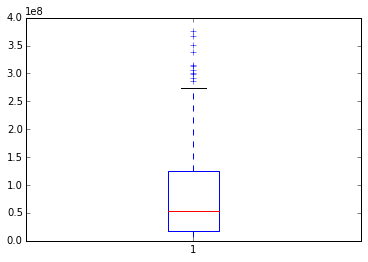
\includegraphics[max size={\textwidth}{\textheight}]{Data_Science_HW_1_files/Data_Science_HW_1_14_9.png}
    \par
    \end{center}
    
            \end{InvisibleVerbatim}
            
                \begin{InvisibleVerbatim}
                \vspace{-0.5\baselineskip}
\begin{alltt}Mean : Median : Mode : Std : Min : Max
(99349241.695473254, 59431365.0, (array([ 6000000.]), array([ 2.])),
96341240.73238185, 691880.0, 381109762.0)
\end{alltt}

            \end{InvisibleVerbatim}
            
                \begin{InvisibleVerbatim}
                \vspace{-0.5\baselineskip}
    \begin{center}
    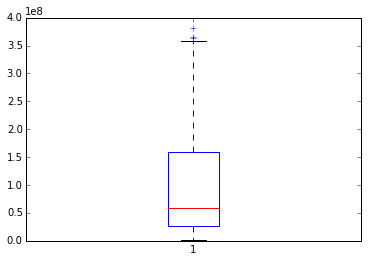
\includegraphics[max size={\textwidth}{\textheight}]{Data_Science_HW_1_files/Data_Science_HW_1_14_11.png}
    \par
    \end{center}
    
            \end{InvisibleVerbatim}
            
        
    
That concludes Problem 1.\section{Problem 2}In problem 2, we look at the correlation between US DVD sales of movies
and their production budgets, again for all movies first and then for
just the top 5 distributors, based on number of movies made this time.

    % Make sure that atleast 4 lines are below the HR
    \needspace{4\baselineskip}

    
        \vspace{6pt}
        \makebox[0.1\linewidth]{\smaller\hfill\tt\color{nbframe-in-prompt}In\hspace{4pt}{[}12{]}:\hspace{4pt}}\\*
        \vspace{-2.65\baselineskip}
        \begin{ColorVerbatim}
            \vspace{-0.7\baselineskip}
            \begin{Verbatim}[commandchars=\\\{\}]
\PY{n}{dvd\PYZus{}sales\PYZus{}i} \PY{o}{=} \PY{l+m+mi}{3}
\PY{n}{prod\PYZus{}bud\PYZus{}i} \PY{o}{=} \PY{l+m+mi}{4}

\PY{n}{overall} \PY{o}{=} \PY{n}{np}\PY{o}{.}\PY{n}{array}\PY{p}{(}\PY{p}{[}\PY{n}{x} \PY{k}{for} \PY{n}{x} \PY{o+ow}{in} \PY{n}{movies}\PY{p}{[}\PY{l+m+mi}{1}\PY{p}{:}\PY{p}{,}\PY{n}{dvd\PYZus{}sales\PYZus{}i}\PY{p}{:}\PY{n}{prod\PYZus{}bud\PYZus{}i}\PY{o}{+}\PY{l+m+mi}{1}\PY{p}{]} \PY{k}{if} \PY{n}{isnum}\PY{p}{(}\PY{n}{x}\PY{p}{[}\PY{l+m+mi}{0}\PY{p}{]}\PY{p}{)} \PY{o+ow}{and} \PY{n}{isnum}\PY{p}{(}\PY{n}{x}\PY{p}{[}\PY{l+m+mi}{1}\PY{p}{]}\PY{p}{)}\PY{p}{]}\PY{p}{)}
\PY{n}{overall\PYZus{}dvd} \PY{o}{=} \PY{n}{stats}\PY{o}{.}\PY{n}{zscore}\PY{p}{(}\PY{n}{np}\PY{o}{.}\PY{n}{array}\PY{p}{(}\PY{n}{overall}\PY{p}{[}\PY{p}{:}\PY{p}{,}\PY{l+m+mi}{0}\PY{p}{]}\PY{p}{)}\PY{o}{.}\PY{n}{astype}\PY{p}{(}\PY{n}{np}\PY{o}{.}\PY{n}{float}\PY{p}{)}\PY{p}{)}
\PY{n}{overall\PYZus{}prod} \PY{o}{=} \PY{n}{stats}\PY{o}{.}\PY{n}{zscore}\PY{p}{(}\PY{n}{np}\PY{o}{.}\PY{n}{array}\PY{p}{(}\PY{n}{overall}\PY{p}{[}\PY{p}{:}\PY{p}{,}\PY{l+m+mi}{1}\PY{p}{]}\PY{p}{)}\PY{o}{.}\PY{n}{astype}\PY{p}{(}\PY{n}{np}\PY{o}{.}\PY{n}{float}\PY{p}{)}\PY{p}{)}
\PY{n}{pearson} \PY{o}{=} \PY{n}{stats}\PY{o}{.}\PY{n}{pearsonr}\PY{p}{(}\PY{n}{overall\PYZus{}dvd}\PY{p}{,} \PY{n}{overall\PYZus{}prod}\PY{p}{)}
\PY{n}{fig} \PY{o}{=} \PY{n}{plt}\PY{o}{.}\PY{n}{figure}\PY{p}{(}\PY{p}{)}
\PY{n}{ax} \PY{o}{=} \PY{n}{fig}\PY{o}{.}\PY{n}{add\PYZus{}subplot}\PY{p}{(}\PY{l+m+mi}{111}\PY{p}{)}
\PY{n}{ax}\PY{o}{.}\PY{n}{scatter}\PY{p}{(}\PY{n}{overall\PYZus{}dvd}\PY{p}{,} \PY{n}{overall\PYZus{}prod}\PY{p}{)}
\PY{n}{plt}\PY{o}{.}\PY{n}{show}\PY{p}{(}\PY{p}{)}
\PY{k}{print} \PY{l+s}{\PYZdq{}}\PY{l+s}{Pearson Coefficient: }\PY{l+s}{\PYZdq{}} \PY{o}{+} \PY{n+nb}{str}\PY{p}{(}\PY{n}{pearson}\PY{p}{)}
\end{Verbatim}

            
                \vspace{-0.2\baselineskip}
            
        \end{ColorVerbatim}
    

    

        % If the first block is an image, minipage the image.  Else
        % request a certain amount of space for the input text.
        \needspace{4\baselineskip}
        
        

            % Add document contents.
            
                \begin{InvisibleVerbatim}
                \vspace{-0.5\baselineskip}
    \begin{center}
    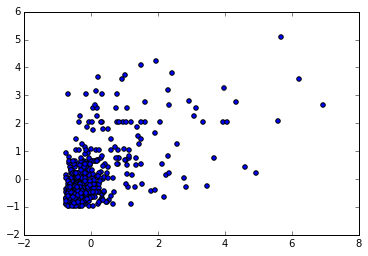
\includegraphics[max size={\textwidth}{\textheight}]{Data_Science_HW_1_files/Data_Science_HW_1_18_0.png}
    \par
    \end{center}
    
            \end{InvisibleVerbatim}
            
                \begin{InvisibleVerbatim}
                \vspace{-0.5\baselineskip}
\begin{alltt}Pearson Coefficient: (0.59202191412497462, 1.5270314436786304e-54)
\end{alltt}

            \end{InvisibleVerbatim}
            
        
    


    % Make sure that atleast 4 lines are below the HR
    \needspace{4\baselineskip}

    
        \vspace{6pt}
        \makebox[0.1\linewidth]{\smaller\hfill\tt\color{nbframe-in-prompt}In\hspace{4pt}{[}56{]}:\hspace{4pt}}\\*
        \vspace{-2.65\baselineskip}
        \begin{ColorVerbatim}
            \vspace{-0.7\baselineskip}
            \begin{Verbatim}[commandchars=\\\{\}]
\PY{n}{dist\PYZus{}num\PYZus{}movies} \PY{o}{=} \PY{p}{[}\PY{p}{[}\PY{n}{dist}\PY{p}{[}\PY{l+m+mi}{0}\PY{p}{]}\PY{p}{,} \PY{n+nb}{len}\PY{p}{(}\PY{n}{dist}\PY{p}{[}\PY{l+m+mi}{1}\PY{p}{]}\PY{p}{)}\PY{p}{]} \PY{k}{for} \PY{n}{dist} \PY{o+ow}{in} \PY{n}{dist\PYZus{}grouped} \PY{k}{if} \PY{n}{dist}\PY{p}{[}\PY{l+m+mi}{0}\PY{p}{]} \PY{o}{!=} \PY{l+s}{\PYZdq{}}\PY{l+s}{\PYZdq{}}\PY{p}{]}
\PY{n}{dist\PYZus{}num\PYZus{}movies}\PY{o}{.}\PY{n}{sort}\PY{p}{(}\PY{n}{key}\PY{o}{=}\PY{k}{lambda} \PY{n}{x}\PY{p}{:} \PY{n}{x}\PY{p}{[}\PY{l+m+mi}{1}\PY{p}{]}\PY{p}{,} \PY{n}{reverse}\PY{o}{=}\PY{n+nb+bp}{True}\PY{p}{)}
\PY{n}{top6\PYZus{}rows} \PY{o}{=} \PY{p}{[}\PY{p}{]}
\PY{k}{print} \PY{l+s}{\PYZdq{}}\PY{l+s}{Top 6 movies are: }\PY{l+s}{\PYZdq{}}
\PY{k}{for} \PY{n}{top} \PY{o+ow}{in} \PY{n}{dist\PYZus{}num\PYZus{}movies}\PY{p}{[}\PY{p}{:}\PY{l+m+mi}{6}\PY{p}{]}\PY{p}{:}
    \PY{k}{print} \PY{n}{top}\PY{p}{[}\PY{l+m+mi}{0}\PY{p}{]}
    \PY{n}{top6\PYZus{}rows}\PY{o}{.}\PY{n}{append}\PY{p}{(}\PY{p}{[}\PY{n}{top}\PY{p}{[}\PY{l+m+mi}{0}\PY{p}{]}\PY{p}{,} \PY{p}{[}\PY{n}{row} \PY{k}{for} \PY{n}{row} \PY{o+ow}{in} \PY{n}{movies} \PY{k}{if} \PY{n}{row}\PY{p}{[}\PY{n}{dist\PYZus{}i}\PY{p}{]} \PY{o}{==} \PY{n}{top}\PY{p}{[}\PY{l+m+mi}{0}\PY{p}{]}\PY{p}{]}\PY{p}{]}\PY{p}{)}
\PY{k}{print} \PY{l+s}{\PYZdq{}}\PY{l+s}{\PYZdq{}}
\PY{k}{for} \PY{n}{dirty\PYZus{}dist} \PY{o+ow}{in} \PY{n}{top6\PYZus{}rows}\PY{p}{:}
    \PY{n}{dist} \PY{o}{=} \PY{n}{np}\PY{o}{.}\PY{n}{array}\PY{p}{(}\PY{n}{dirty\PYZus{}dist}\PY{p}{[}\PY{l+m+mi}{1}\PY{p}{:}\PY{p}{]}\PY{p}{[}\PY{l+m+mi}{0}\PY{p}{]}\PY{p}{)}
    \PY{n}{overall} \PY{o}{=} \PY{n}{np}\PY{o}{.}\PY{n}{array}\PY{p}{(}\PY{p}{[}\PY{n}{x} \PY{k}{for} \PY{n}{x} \PY{o+ow}{in} \PY{n}{dist}\PY{p}{[}\PY{l+m+mi}{1}\PY{p}{:}\PY{p}{,}\PY{n}{dvd\PYZus{}sales\PYZus{}i}\PY{p}{:}\PY{n}{prod\PYZus{}bud\PYZus{}i}\PY{o}{+}\PY{l+m+mi}{1}\PY{p}{]} \PY{k}{if} \PY{n}{isnum}\PY{p}{(}\PY{n}{x}\PY{p}{[}\PY{l+m+mi}{0}\PY{p}{]}\PY{p}{)} \PY{o+ow}{and} \PY{n}{isnum}\PY{p}{(}\PY{n}{x}\PY{p}{[}\PY{l+m+mi}{1}\PY{p}{]}\PY{p}{)}\PY{p}{]}\PY{p}{)}
    \PY{n}{overall\PYZus{}dvd} \PY{o}{=} \PY{n}{stats}\PY{o}{.}\PY{n}{zscore}\PY{p}{(}\PY{n}{np}\PY{o}{.}\PY{n}{array}\PY{p}{(}\PY{n}{overall}\PY{p}{[}\PY{p}{:}\PY{p}{,}\PY{l+m+mi}{0}\PY{p}{]}\PY{p}{)}\PY{o}{.}\PY{n}{astype}\PY{p}{(}\PY{n}{np}\PY{o}{.}\PY{n}{float}\PY{p}{)}\PY{p}{)}
    \PY{n}{overall\PYZus{}prod} \PY{o}{=} \PY{n}{stats}\PY{o}{.}\PY{n}{zscore}\PY{p}{(}\PY{n}{np}\PY{o}{.}\PY{n}{array}\PY{p}{(}\PY{n}{overall}\PY{p}{[}\PY{p}{:}\PY{p}{,}\PY{l+m+mi}{1}\PY{p}{]}\PY{p}{)}\PY{o}{.}\PY{n}{astype}\PY{p}{(}\PY{n}{np}\PY{o}{.}\PY{n}{float}\PY{p}{)}\PY{p}{)}
    \PY{n}{pearson} \PY{o}{=} \PY{n}{stats}\PY{o}{.}\PY{n}{pearsonr}\PY{p}{(}\PY{n}{overall\PYZus{}dvd}\PY{p}{,} \PY{n}{overall\PYZus{}prod}\PY{p}{)}
    \PY{n}{fig} \PY{o}{=} \PY{n}{plt}\PY{o}{.}\PY{n}{figure}\PY{p}{(}\PY{p}{)}
    \PY{n}{ax} \PY{o}{=} \PY{n}{fig}\PY{o}{.}\PY{n}{add\PYZus{}subplot}\PY{p}{(}\PY{l+m+mi}{111}\PY{p}{)}
    \PY{n}{ax}\PY{o}{.}\PY{n}{scatter}\PY{p}{(}\PY{n}{overall\PYZus{}dvd}\PY{p}{,} \PY{n}{overall\PYZus{}prod}\PY{p}{)}
    \PY{n}{plt}\PY{o}{.}\PY{n}{show}\PY{p}{(}\PY{p}{)}
    \PY{k}{print} \PY{l+s}{\PYZdq{}}\PY{l+s}{Pearson Coefficient for }\PY{l+s}{\PYZdq{}} \PY{o}{+} \PY{n+nb}{str}\PY{p}{(}\PY{n}{dirty\PYZus{}dist}\PY{p}{[}\PY{l+m+mi}{0}\PY{p}{]}\PY{p}{)} \PY{o}{+} \PY{l+s}{\PYZdq{}}\PY{l+s}{ is }\PY{l+s}{\PYZdq{}} \PY{o}{+} \PY{n+nb}{str}\PY{p}{(}\PY{n}{pearson}\PY{p}{)}
            
\end{Verbatim}

            
                \vspace{-0.2\baselineskip}
            
        \end{ColorVerbatim}
    

    

        % If the first block is an image, minipage the image.  Else
        % request a certain amount of space for the input text.
        \needspace{4\baselineskip}
        
        

            % Add document contents.
            
                \begin{InvisibleVerbatim}
                \vspace{-0.5\baselineskip}
\begin{alltt}Top 6 movies are:
Warner Bros.
Sony Pictures
Paramount Pictures
Universal
Walt Disney Pictures
20th Century Fox

\end{alltt}

            \end{InvisibleVerbatim}
            
                \begin{InvisibleVerbatim}
                \vspace{-0.5\baselineskip}
    \begin{center}
    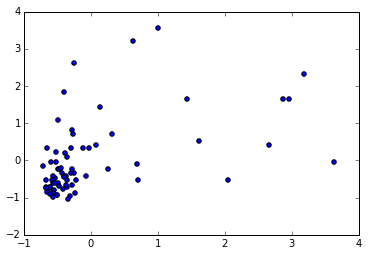
\includegraphics[max size={\textwidth}{\textheight}]{Data_Science_HW_1_files/Data_Science_HW_1_19_1.png}
    \par
    \end{center}
    
            \end{InvisibleVerbatim}
            
                \begin{InvisibleVerbatim}
                \vspace{-0.5\baselineskip}
\begin{alltt}Pearson Coefficient for Warner Bros. is (0.48907060955392062,
1.5062835928126968e-05)
\end{alltt}

            \end{InvisibleVerbatim}
            
                \begin{InvisibleVerbatim}
                \vspace{-0.5\baselineskip}
    \begin{center}
    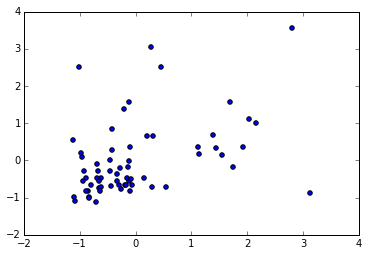
\includegraphics[max size={\textwidth}{\textheight}]{Data_Science_HW_1_files/Data_Science_HW_1_19_3.png}
    \par
    \end{center}
    
            \end{InvisibleVerbatim}
            
                \begin{InvisibleVerbatim}
                \vspace{-0.5\baselineskip}
\begin{alltt}Pearson Coefficient for Sony Pictures is (0.4150080481425103,
0.000650109845788543)
\end{alltt}

            \end{InvisibleVerbatim}
            
                \begin{InvisibleVerbatim}
                \vspace{-0.5\baselineskip}
    \begin{center}
    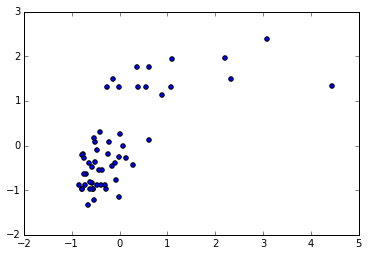
\includegraphics[max size={\textwidth}{\textheight}]{Data_Science_HW_1_files/Data_Science_HW_1_19_5.png}
    \par
    \end{center}
    
            \end{InvisibleVerbatim}
            
                \begin{InvisibleVerbatim}
                \vspace{-0.5\baselineskip}
\begin{alltt}Pearson Coefficient for Paramount Pictures is (0.71037449047412604,
1.2428382567834893e-09)
\end{alltt}

            \end{InvisibleVerbatim}
            
                \begin{InvisibleVerbatim}
                \vspace{-0.5\baselineskip}
    \begin{center}
    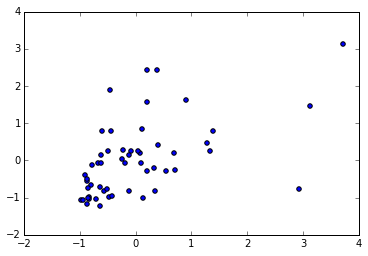
\includegraphics[max size={\textwidth}{\textheight}]{Data_Science_HW_1_files/Data_Science_HW_1_19_7.png}
    \par
    \end{center}
    
            \end{InvisibleVerbatim}
            
                \begin{InvisibleVerbatim}
                \vspace{-0.5\baselineskip}
\begin{alltt}Pearson Coefficient for Universal is (0.5336537644887257,
3.2478783794672723e-05)
\end{alltt}

            \end{InvisibleVerbatim}
            
                \begin{InvisibleVerbatim}
                \vspace{-0.5\baselineskip}
    \begin{center}
    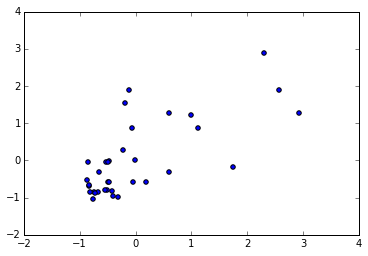
\includegraphics[max size={\textwidth}{\textheight}]{Data_Science_HW_1_files/Data_Science_HW_1_19_9.png}
    \par
    \end{center}
    
            \end{InvisibleVerbatim}
            
                \begin{InvisibleVerbatim}
                \vspace{-0.5\baselineskip}
\begin{alltt}Pearson Coefficient for Walt Disney Pictures is (0.70717349840013533,
2.0410608002334782e-06)
\end{alltt}

            \end{InvisibleVerbatim}
            
                \begin{InvisibleVerbatim}
                \vspace{-0.5\baselineskip}
    \begin{center}
    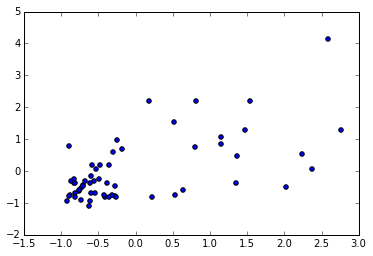
\includegraphics[max size={\textwidth}{\textheight}]{Data_Science_HW_1_files/Data_Science_HW_1_19_11.png}
    \par
    \end{center}
    
            \end{InvisibleVerbatim}
            
                \begin{InvisibleVerbatim}
                \vspace{-0.5\baselineskip}
\begin{alltt}Pearson Coefficient for 20th Century Fox is (0.60664000034943655,
4.4747831117473855e-07)
\end{alltt}

            \end{InvisibleVerbatim}
            
        
    
There's definitely \emph{a} correlation between DVD sales and Production
Budget, but it varies between firms from between 0.4 and 0.7, so between
moderate-low to moderate-high.\section{Problem 3}First for this problem, we need to normalize all of the data.I use min/max scaling for numeric data to bring everything onto a
{[}0,1{]} scale.

    % Make sure that atleast 4 lines are below the HR
    \needspace{4\baselineskip}

    
        \vspace{6pt}
        \makebox[0.1\linewidth]{\smaller\hfill\tt\color{nbframe-in-prompt}In\hspace{4pt}{[}21{]}:\hspace{4pt}}\\*
        \vspace{-2.65\baselineskip}
        \begin{ColorVerbatim}
            \vspace{-0.7\baselineskip}
            \begin{Verbatim}[commandchars=\\\{\}]
\PY{c}{\PYZsh{}Normalize metrics \PYZhy{} min\PYZhy{}max normalize}

\PY{n}{dist\PYZus{}i} \PY{o}{=} \PY{l+m+mi}{8}
\PY{n}{source\PYZus{}i} \PY{o}{=} \PY{l+m+mi}{9}
\PY{n}{genre\PYZus{}i} \PY{o}{=} \PY{l+m+mi}{10}

\PY{k}{def} \PY{n+nf}{float\PYZus{}equal}\PY{p}{(}\PY{n}{x1}\PY{p}{,} \PY{n}{x2}\PY{p}{)}\PY{p}{:}
    \PY{k}{return} \PY{n+nb}{abs}\PY{p}{(}\PY{n}{x1} \PY{o}{\PYZhy{}} \PY{n}{x2}\PY{p}{)} \PY{o}{\PYZlt{}}\PY{o}{=}\PY{l+m+mf}{0.001}

\PY{n}{imdb\PYZus{}votes\PYZus{}i} \PY{o}{=} \PY{n+nb}{len}\PY{p}{(}\PY{n}{movies}\PY{p}{[}\PY{l+m+mi}{0}\PY{p}{]}\PY{p}{)} \PY{o}{\PYZhy{}}\PY{l+m+mi}{1}
\PY{n}{imdb\PYZus{}rating\PYZus{}i} \PY{o}{=} \PY{n}{imdb\PYZus{}votes\PYZus{}i} \PY{o}{\PYZhy{}}\PY{l+m+mi}{1}
\PY{n}{rotten\PYZus{}i} \PY{o}{=} \PY{n}{imdb\PYZus{}votes\PYZus{}i} \PY{o}{\PYZhy{}} \PY{l+m+mi}{2}
\PY{k}{def} \PY{n+nf}{normalizeRatings}\PY{p}{(}\PY{n}{movies}\PY{p}{)}\PY{p}{:}
    
    \PY{n}{votes} \PY{o}{=} \PY{n}{np}\PY{o}{.}\PY{n}{array}\PY{p}{(}\PY{p}{[}\PY{n}{x} \PY{k}{if} \PY{n}{isnum}\PY{p}{(}\PY{n}{x}\PY{p}{)} \PY{k}{else} \PY{l+m+mf}{0.00000} \PY{k}{for} \PY{n}{x} \PY{o+ow}{in} \PY{n}{movies}\PY{p}{[}\PY{p}{:}\PY{p}{,}\PY{n}{imdb\PYZus{}votes\PYZus{}i}\PY{p}{]}\PY{p}{]}\PY{p}{)}\PY{o}{.}\PY{n}{astype}\PY{p}{(}\PY{n}{np}\PY{o}{.}\PY{n}{float}\PY{p}{)}
    \PY{n}{im\PYZus{}ratings} \PY{o}{=} \PY{n}{np}\PY{o}{.}\PY{n}{array}\PY{p}{(}\PY{p}{[}\PY{n}{x} \PY{k}{if} \PY{n}{isnum}\PY{p}{(}\PY{n}{x}\PY{p}{)} \PY{k}{else} \PY{l+m+mi}{0} \PY{k}{for} \PY{n}{x} \PY{o+ow}{in} \PY{n}{movies}\PY{p}{[}\PY{p}{:}\PY{p}{,}\PY{n}{imdb\PYZus{}rating\PYZus{}i}\PY{p}{]}\PY{p}{]}\PY{p}{)}\PY{o}{.}\PY{n}{astype}\PY{p}{(}\PY{n}{np}\PY{o}{.}\PY{n}{float}\PY{p}{)}
    \PY{n}{rotten\PYZus{}ratings} \PY{o}{=} \PY{n}{np}\PY{o}{.}\PY{n}{array}\PY{p}{(}\PY{p}{[}\PY{n}{x} \PY{k}{if} \PY{n}{isnum}\PY{p}{(}\PY{n}{x}\PY{p}{)} \PY{k}{else} \PY{l+m+mi}{0} \PY{k}{for} \PY{n}{x} \PY{o+ow}{in} \PY{n}{movies}\PY{p}{[}\PY{p}{:}\PY{p}{,}\PY{n}{rotten\PYZus{}i}\PY{p}{]}\PY{p}{]}\PY{p}{)}\PY{o}{.}\PY{n}{astype}\PY{p}{(}\PY{n}{np}\PY{o}{.}\PY{n}{float}\PY{p}{)}
    \PY{k}{print} \PY{n}{votes}
    
    \PY{n}{voteMean} \PY{o}{=} \PY{n}{np}\PY{o}{.}\PY{n}{mean}\PY{p}{(}\PY{p}{[}\PY{n}{x} \PY{k}{for} \PY{n}{x} \PY{o+ow}{in} \PY{n}{votes} \PY{k}{if} \PY{o+ow}{not} \PY{n}{float\PYZus{}equal}\PY{p}{(}\PY{n}{x}\PY{p}{,}\PY{l+m+mi}{0}\PY{p}{)}\PY{p}{]}\PY{p}{)}
    \PY{n}{imMean} \PY{o}{=} \PY{n}{np}\PY{o}{.}\PY{n}{mean}\PY{p}{(}\PY{p}{[}\PY{n}{x} \PY{k}{for} \PY{n}{x} \PY{o+ow}{in} \PY{n}{im\PYZus{}ratings} \PY{k}{if} \PY{o+ow}{not} \PY{n}{float\PYZus{}equal}\PY{p}{(}\PY{n}{x}\PY{p}{,}\PY{l+m+mi}{0}\PY{p}{)}\PY{p}{]}\PY{p}{)}
    \PY{n}{rottenMean} \PY{o}{=} \PY{n}{np}\PY{o}{.}\PY{n}{mean}\PY{p}{(}\PY{p}{[}\PY{n}{x} \PY{k}{for} \PY{n}{x} \PY{o+ow}{in} \PY{n}{rotten\PYZus{}ratings} \PY{k}{if} \PY{o+ow}{not} \PY{n}{float\PYZus{}equal}\PY{p}{(}\PY{n}{x}\PY{p}{,}\PY{l+m+mi}{0}\PY{p}{)}\PY{p}{]}\PY{p}{)}
    
    \PY{k}{print} \PY{l+s}{\PYZdq{}}\PY{l+s}{Vote : IMBD Rating : Rotten Rating Means}\PY{l+s}{\PYZdq{}}
    \PY{k}{print} \PY{n+nb}{str}\PY{p}{(}\PY{n}{voteMean}\PY{p}{)} \PY{o}{+} \PY{l+s}{\PYZdq{}}\PY{l+s}{ : }\PY{l+s}{\PYZdq{}} \PY{o}{+} \PY{n+nb}{str}\PY{p}{(}\PY{n}{imMean}\PY{p}{)} \PY{o}{+} \PY{l+s}{\PYZdq{}}\PY{l+s}{ : }\PY{l+s}{\PYZdq{}} \PY{o}{+} \PY{n+nb}{str}\PY{p}{(}\PY{n}{rottenMean}\PY{p}{)}
    
    \PY{n}{votes} \PY{o}{=} \PY{n}{np}\PY{o}{.}\PY{n}{array}\PY{p}{(}\PY{p}{[}\PY{n}{x} \PY{k}{if} \PY{o+ow}{not} \PY{n}{float\PYZus{}equal}\PY{p}{(}\PY{n}{x}\PY{p}{,}\PY{l+m+mi}{0}\PY{p}{)} \PY{k}{else} \PY{n}{voteMean} \PY{k}{for} \PY{n}{x} \PY{o+ow}{in} \PY{n}{votes}\PY{p}{]}\PY{p}{)}
    \PY{n}{im\PYZus{}ratings} \PY{o}{=} \PY{n}{np}\PY{o}{.}\PY{n}{array}\PY{p}{(}\PY{p}{[}\PY{n}{x} \PY{k}{if} \PY{o+ow}{not} \PY{n}{float\PYZus{}equal}\PY{p}{(}\PY{n}{x}\PY{p}{,}\PY{l+m+mi}{0}\PY{p}{)} \PY{k}{else} \PY{n}{imMean} \PY{k}{for} \PY{n}{x} \PY{o+ow}{in} \PY{n}{im\PYZus{}ratings}\PY{p}{]}\PY{p}{)}
    \PY{n}{rotten\PYZus{}ratings} \PY{o}{=} \PY{n}{np}\PY{o}{.}\PY{n}{array}\PY{p}{(}\PY{p}{[}\PY{n}{x} \PY{k}{if} \PY{o+ow}{not} \PY{n}{float\PYZus{}equal}\PY{p}{(}\PY{n}{x}\PY{p}{,}\PY{l+m+mi}{0}\PY{p}{)} \PY{k}{else} \PY{n}{rottenMean} \PY{k}{for} \PY{n}{x} \PY{o+ow}{in} \PY{n}{rotten\PYZus{}ratings}\PY{p}{]}\PY{p}{)}
    
    \PY{n}{minVotes} \PY{o}{=} \PY{n+nb}{min}\PY{p}{(}\PY{n}{votes}\PY{p}{)}
    \PY{n}{maxVotes} \PY{o}{=} \PY{n+nb}{max}\PY{p}{(}\PY{n}{votes}\PY{p}{)}
    \PY{n}{minRotten} \PY{o}{=} \PY{n+nb}{min}\PY{p}{(}\PY{n}{rotten\PYZus{}ratings}\PY{p}{)}
    \PY{n}{maxRotten} \PY{o}{=} \PY{n+nb}{max}\PY{p}{(}\PY{n}{rotten\PYZus{}ratings}\PY{p}{)}
    \PY{n}{minImbdRating} \PY{o}{=} \PY{n+nb}{min}\PY{p}{(}\PY{n}{im\PYZus{}ratings}\PY{p}{)}
    \PY{n}{maxImbdRating} \PY{o}{=} \PY{n+nb}{max}\PY{p}{(}\PY{n}{im\PYZus{}ratings}\PY{p}{)}
    
    \PY{k}{for} \PY{n}{i}\PY{p}{,} \PY{n}{movie} \PY{o+ow}{in} \PY{n+nb}{enumerate}\PY{p}{(}\PY{n}{movies}\PY{p}{)}\PY{p}{:}
        \PY{n}{movie}\PY{p}{[}\PY{n}{imdb\PYZus{}votes\PYZus{}i}\PY{p}{]} \PY{o}{=} \PY{n+nb}{float}\PY{p}{(}\PY{n}{votes}\PY{p}{[}\PY{n}{i}\PY{p}{]} \PY{o}{\PYZhy{}} \PY{n}{minVotes}\PY{p}{)} \PY{o}{/} \PY{n+nb}{float}\PY{p}{(}\PY{n}{maxVotes} \PY{o}{\PYZhy{}} \PY{n}{minVotes}\PY{p}{)}
        \PY{n}{movie}\PY{p}{[}\PY{n}{imdb\PYZus{}rating\PYZus{}i}\PY{p}{]} \PY{o}{=} \PY{n+nb}{float}\PY{p}{(}\PY{n}{im\PYZus{}ratings}\PY{p}{[}\PY{n}{i}\PY{p}{]} \PY{o}{\PYZhy{}} \PY{n}{minImbdRating}\PY{p}{)} \PY{o}{/} \PY{n+nb}{float}\PY{p}{(}\PY{n}{maxImbdRating} \PY{o}{\PYZhy{}} \PY{n}{minImbdRating}\PY{p}{)}
        \PY{n}{movie}\PY{p}{[}\PY{n}{rotten\PYZus{}i}\PY{p}{]} \PY{o}{=} \PY{n+nb}{float}\PY{p}{(}\PY{n}{rotten\PYZus{}ratings}\PY{p}{[}\PY{n}{i}\PY{p}{]} \PY{o}{\PYZhy{}} \PY{n}{minRotten}\PY{p}{)} \PY{o}{/} \PY{n+nb}{float}\PY{p}{(}\PY{n}{maxRotten} \PY{o}{\PYZhy{}} \PY{n}{minRotten}\PY{p}{)}
    
    \PY{k}{return} \PY{n}{movies}
\end{Verbatim}

            
                \vspace{-0.2\baselineskip}
            
        \end{ColorVerbatim}
    
No special normalization here, just min/max scaling.

    % Make sure that atleast 4 lines are below the HR
    \needspace{4\baselineskip}

    
        \vspace{6pt}
        \makebox[0.1\linewidth]{\smaller\hfill\tt\color{nbframe-in-prompt}In\hspace{4pt}{[}{]}:\hspace{4pt}}\\*
        \vspace{-2.65\baselineskip}
        \begin{ColorVerbatim}
            \vspace{-0.7\baselineskip}
            \begin{Verbatim}[commandchars=\\\{\}]
\PY{n}{us\PYZus{}i} \PY{o}{=} \PY{l+m+mi}{1}
\PY{n}{world\PYZus{}i} \PY{o}{=} \PY{l+m+mi}{2}
\PY{n}{dvd\PYZus{}i} \PY{o}{=} \PY{l+m+mi}{3}
\PY{k}{def} \PY{n+nf}{normalizeRevenues}\PY{p}{(}\PY{n}{movies}\PY{p}{)}\PY{p}{:}
    
    \PY{n}{usGross} \PY{o}{=} \PY{n}{np}\PY{o}{.}\PY{n}{array}\PY{p}{(}\PY{p}{[}\PY{n}{x} \PY{k}{if} \PY{n}{isnum}\PY{p}{(}\PY{n}{x}\PY{p}{)} \PY{k}{else} \PY{l+m+mi}{0} \PY{k}{for} \PY{n}{x} \PY{o+ow}{in} \PY{n}{movies}\PY{p}{[}\PY{p}{:}\PY{p}{,}\PY{n}{us\PYZus{}i}\PY{p}{]}\PY{p}{]}\PY{p}{)}\PY{o}{.}\PY{n}{astype}\PY{p}{(}\PY{n}{np}\PY{o}{.}\PY{n}{float}\PY{p}{)}
    \PY{n}{worldGross} \PY{o}{=} \PY{n}{np}\PY{o}{.}\PY{n}{array}\PY{p}{(}\PY{p}{[}\PY{n}{x} \PY{k}{if} \PY{n}{isnum}\PY{p}{(}\PY{n}{x}\PY{p}{)} \PY{k}{else} \PY{l+m+mi}{0} \PY{k}{for} \PY{n}{x} \PY{o+ow}{in} \PY{n}{movies}\PY{p}{[}\PY{p}{:}\PY{p}{,}\PY{n}{world\PYZus{}i}\PY{p}{]}\PY{p}{]}\PY{p}{)}\PY{o}{.}\PY{n}{astype}\PY{p}{(}\PY{n}{np}\PY{o}{.}\PY{n}{float}\PY{p}{)}
    \PY{n}{dvdSales} \PY{o}{=} \PY{n}{np}\PY{o}{.}\PY{n}{array}\PY{p}{(}\PY{p}{[}\PY{n}{x} \PY{k}{if} \PY{n}{isnum}\PY{p}{(}\PY{n}{x}\PY{p}{)} \PY{k}{else} \PY{l+m+mi}{0} \PY{k}{for} \PY{n}{x} \PY{o+ow}{in} \PY{n}{movies}\PY{p}{[}\PY{p}{:}\PY{p}{,}\PY{n}{dvd\PYZus{}i}\PY{p}{]}\PY{p}{]}\PY{p}{)}\PY{o}{.}\PY{n}{astype}\PY{p}{(}\PY{n}{np}\PY{o}{.}\PY{n}{float}\PY{p}{)}
    
    \PY{n}{usMean} \PY{o}{=} \PY{n}{np}\PY{o}{.}\PY{n}{mean}\PY{p}{(}\PY{p}{[}\PY{n}{x} \PY{k}{for} \PY{n}{x} \PY{o+ow}{in} \PY{n}{usGross} \PY{k}{if} \PY{o+ow}{not} \PY{n}{float\PYZus{}equal}\PY{p}{(}\PY{n}{x}\PY{p}{,}\PY{l+m+mi}{0}\PY{p}{)}\PY{p}{]}\PY{p}{)}
    \PY{n}{worldMean} \PY{o}{=} \PY{n}{np}\PY{o}{.}\PY{n}{mean}\PY{p}{(}\PY{p}{[}\PY{n}{x} \PY{k}{for} \PY{n}{x} \PY{o+ow}{in} \PY{n}{worldGross} \PY{k}{if} \PY{o+ow}{not} \PY{n}{float\PYZus{}equal}\PY{p}{(}\PY{n}{x}\PY{p}{,}\PY{l+m+mi}{0}\PY{p}{)}\PY{p}{]}\PY{p}{)}
    \PY{n}{dvdMean} \PY{o}{=} \PY{n}{np}\PY{o}{.}\PY{n}{mean}\PY{p}{(}\PY{p}{[}\PY{n}{x} \PY{k}{for} \PY{n}{x} \PY{o+ow}{in} \PY{n}{dvdSales} \PY{k}{if} \PY{o+ow}{not} \PY{n}{float\PYZus{}equal}\PY{p}{(}\PY{n}{x}\PY{p}{,}\PY{l+m+mi}{0}\PY{p}{)}\PY{p}{]}\PY{p}{)}
    
    \PY{k}{print} \PY{l+s}{\PYZdq{}}\PY{l+s}{US Gross : World Gross : DVD}\PY{l+s}{\PYZdq{}}
    \PY{k}{print} \PY{n+nb}{str}\PY{p}{(}\PY{n}{usMean}\PY{p}{)} \PY{o}{+} \PY{l+s}{\PYZdq{}}\PY{l+s}{ : }\PY{l+s}{\PYZdq{}} \PY{o}{+} \PY{n+nb}{str}\PY{p}{(}\PY{n}{worldMean}\PY{p}{)} \PY{o}{+} \PY{l+s}{\PYZdq{}}\PY{l+s}{ : }\PY{l+s}{\PYZdq{}} \PY{o}{+} \PY{n+nb}{str}\PY{p}{(}\PY{n}{dvdMean}\PY{p}{)}
    
    \PY{n}{usGross} \PY{o}{=} \PY{n}{np}\PY{o}{.}\PY{n}{array}\PY{p}{(}\PY{p}{[}\PY{n}{x} \PY{k}{if} \PY{o+ow}{not} \PY{n}{float\PYZus{}equal}\PY{p}{(}\PY{n}{x}\PY{p}{,}\PY{l+m+mi}{0}\PY{p}{)} \PY{k}{else} \PY{n}{usMean} \PY{k}{for} \PY{n}{x} \PY{o+ow}{in} \PY{n}{usGross}\PY{p}{]}\PY{p}{)}


    \PY{n}{worldGross} \PY{o}{=} \PY{n}{np}\PY{o}{.}\PY{n}{array}\PY{p}{(}\PY{p}{[}\PY{n}{x} \PY{k}{if} \PY{o+ow}{not} \PY{n}{float\PYZus{}equal}\PY{p}{(}\PY{n}{x}\PY{p}{,}\PY{l+m+mi}{0}\PY{p}{)} \PY{k}{else} \PY{n}{worldMean} \PY{k}{for} \PY{n}{x} \PY{o+ow}{in} \PY{n}{worldGross}\PY{p}{]}\PY{p}{)}
    \PY{n}{dvdSales} \PY{o}{=} \PY{n}{np}\PY{o}{.}\PY{n}{array}\PY{p}{(}\PY{p}{[}\PY{n}{x} \PY{k}{if} \PY{o+ow}{not} \PY{n}{float\PYZus{}equal}\PY{p}{(}\PY{n}{x}\PY{p}{,}\PY{l+m+mi}{0}\PY{p}{)} \PY{k}{else} \PY{n}{dvdMean} \PY{k}{for} \PY{n}{x} \PY{o+ow}{in} \PY{n}{dvdSales}\PY{p}{]}\PY{p}{)}
    
    \PY{n}{minUs} \PY{o}{=} \PY{n+nb}{min}\PY{p}{(}\PY{n}{usGross}\PY{p}{)}
    \PY{n}{maxUs} \PY{o}{=} \PY{n+nb}{max}\PY{p}{(}\PY{n}{usGross}\PY{p}{)}
    \PY{n}{minWorld} \PY{o}{=} \PY{n+nb}{min}\PY{p}{(}\PY{n}{worldGross}\PY{p}{)}
    \PY{n}{maxWorld} \PY{o}{=} \PY{n+nb}{max}\PY{p}{(}\PY{n}{worldGross}\PY{p}{)}
    \PY{n}{minDvd} \PY{o}{=} \PY{n+nb}{min}\PY{p}{(}\PY{n}{dvdSales}\PY{p}{)}
    \PY{n}{maxDvd} \PY{o}{=} \PY{n+nb}{max}\PY{p}{(}\PY{n}{dvdSales}\PY{p}{)}
    
    \PY{k}{for} \PY{n}{i}\PY{p}{,} \PY{n}{movie} \PY{o+ow}{in} \PY{n+nb}{enumerate}\PY{p}{(}\PY{n}{movies}\PY{p}{)}\PY{p}{:}
        \PY{n}{movie}\PY{p}{[}\PY{n}{us\PYZus{}i}\PY{p}{]} \PY{o}{=} \PY{n+nb}{float}\PY{p}{(}\PY{n}{usGross}\PY{p}{[}\PY{n}{i}\PY{p}{]} \PY{o}{\PYZhy{}} \PY{n}{minUs}\PY{p}{)} \PY{o}{/} \PY{n+nb}{float}\PY{p}{(}\PY{n}{maxUs} \PY{o}{\PYZhy{}} \PY{n}{minUs}\PY{p}{)}
        \PY{n}{movie}\PY{p}{[}\PY{n}{world\PYZus{}i}\PY{p}{]} \PY{o}{=} \PY{n+nb}{float}\PY{p}{(}\PY{n}{worldGross}\PY{p}{[}\PY{n}{i}\PY{p}{]} \PY{o}{\PYZhy{}} \PY{n}{minWorld}\PY{p}{)} \PY{o}{/} \PY{n+nb}{float}\PY{p}{(}\PY{n}{maxWorld} \PY{o}{\PYZhy{}} \PY{n}{minWorld}\PY{p}{)}
        \PY{n}{movie}\PY{p}{[}\PY{n}{dvd\PYZus{}i}\PY{p}{]} \PY{o}{=} \PY{n+nb}{float}\PY{p}{(}\PY{n}{dvdSales}\PY{p}{[}\PY{n}{i}\PY{p}{]} \PY{o}{\PYZhy{}} \PY{n}{minDvd}\PY{p}{)} \PY{o}{/} \PY{n+nb}{float}\PY{p}{(}\PY{n}{maxDvd} \PY{o}{\PYZhy{}} \PY{n}{minDvd}\PY{p}{)}
    
    \PY{k}{return} \PY{n}{movies}
    
    
\end{Verbatim}

            
                \vspace{-0.2\baselineskip}
            
        \end{ColorVerbatim}
    
Normalization here, other than the typical min/max norm only involved
converting the MPAA ratings into an ordinal scale. For MPAA rating, I
convert it into an ordinal variable with G on one end and NC-17 at the
other, implying a G movie is more similar to a PG movie than it is to an
R movie.

    % Make sure that atleast 4 lines are below the HR
    \needspace{4\baselineskip}

    
        \vspace{6pt}
        \makebox[0.1\linewidth]{\smaller\hfill\tt\color{nbframe-in-prompt}In\hspace{4pt}{[}{]}:\hspace{4pt}}\\*
        \vspace{-2.65\baselineskip}
        \begin{ColorVerbatim}
            \vspace{-0.7\baselineskip}
            \begin{Verbatim}[commandchars=\\\{\}]
\PY{n}{mpaa\PYZus{}i} \PY{o}{=} \PY{l+m+mi}{6}
\PY{n}{runtime\PYZus{}i} \PY{o}{=} \PY{l+m+mi}{7}
\PY{k}{def} \PY{n+nf}{normalizeGeneral}\PY{p}{(}\PY{n}{movies}\PY{p}{)}\PY{p}{:}
    \PY{n}{runTimes} \PY{o}{=} \PY{n}{np}\PY{o}{.}\PY{n}{array}\PY{p}{(}\PY{p}{[}\PY{n}{x} \PY{k}{if} \PY{n}{isnum}\PY{p}{(}\PY{n}{x}\PY{p}{)} \PY{k}{else} \PY{l+m+mi}{0} \PY{k}{for} \PY{n}{x} \PY{o+ow}{in} \PY{n}{movies}\PY{p}{[}\PY{p}{:}\PY{p}{,}\PY{n}{runtime\PYZus{}i}\PY{p}{]}\PY{p}{]}\PY{p}{)}\PY{o}{.}\PY{n}{astype}\PY{p}{(}\PY{n}{np}\PY{o}{.}\PY{n}{float}\PY{p}{)}
    
    \PY{n}{runTimeMean} \PY{o}{=} \PY{n}{np}\PY{o}{.}\PY{n}{mean}\PY{p}{(}\PY{p}{[}\PY{n}{x} \PY{k}{for} \PY{n}{x} \PY{o+ow}{in} \PY{n}{runTimes} \PY{k}{if} \PY{o+ow}{not} \PY{n}{float\PYZus{}equal}\PY{p}{(}\PY{n}{x}\PY{p}{,}\PY{l+m+mi}{0}\PY{p}{)}\PY{p}{]}\PY{p}{)}
    \PY{k}{print} \PY{l+s}{\PYZdq{}}\PY{l+s}{RuntimeMean: }\PY{l+s}{\PYZdq{}} \PY{o}{+} \PY{n+nb}{str}\PY{p}{(}\PY{n}{runTimeMean}\PY{p}{)}
    
    \PY{n}{runTimes} \PY{o}{=} \PY{n}{np}\PY{o}{.}\PY{n}{array}\PY{p}{(}\PY{p}{[}\PY{n}{x} \PY{k}{if} \PY{o+ow}{not} \PY{n}{float\PYZus{}equal}\PY{p}{(}\PY{n}{x}\PY{p}{,}\PY{l+m+mi}{0}\PY{p}{)} \PY{k}{else} \PY{n}{runTimeMean} \PY{k}{for} \PY{n}{x} \PY{o+ow}{in} \PY{n}{runTimes}\PY{p}{]}\PY{p}{)}
    \PY{n}{minRuntime} \PY{o}{=} \PY{n+nb}{min}\PY{p}{(}\PY{n}{runTimes}\PY{p}{)}
    \PY{n}{maxRuntime} \PY{o}{=} \PY{n+nb}{max}\PY{p}{(}\PY{n}{runTimes}\PY{p}{)}
    
    \PY{k}{for} \PY{n}{i}\PY{p}{,} \PY{n}{movie} \PY{o+ow}{in} \PY{n+nb}{enumerate}\PY{p}{(}\PY{n}{movies}\PY{p}{)}\PY{p}{:}
        \PY{n}{movie}\PY{p}{[}\PY{n}{mpaa\PYZus{}i}\PY{p}{]} \PY{o}{=} \PY{p}{\PYZob{}}
                         \PY{l+s}{\PYZsq{}}\PY{l+s}{G}\PY{l+s}{\PYZsq{}}\PY{p}{:} \PY{l+m+mf}{0.0}\PY{p}{,}
                         \PY{l+s}{\PYZsq{}}\PY{l+s}{PG}\PY{l+s}{\PYZsq{}}\PY{p}{:} \PY{o}{.}\PY{l+m+mi}{25}\PY{p}{,}
                         \PY{l+s}{\PYZsq{}}\PY{l+s}{PG\PYZhy{}13}\PY{l+s}{\PYZsq{}}\PY{p}{:} \PY{o}{.}\PY{l+m+mi}{5}\PY{p}{,}
                         \PY{l+s}{\PYZsq{}}\PY{l+s}{R}\PY{l+s}{\PYZsq{}}\PY{p}{:} \PY{o}{.}\PY{l+m+mi}{75}\PY{p}{,}
                         \PY{l+s}{\PYZsq{}}\PY{l+s}{NC\PYZhy{}17}\PY{l+s}{\PYZsq{}}\PY{p}{:} \PY{l+m+mf}{1.0}\PY{p}{,}
                         \PY{l+s}{\PYZsq{}}\PY{l+s}{Not Rated}\PY{l+s}{\PYZsq{}}\PY{p}{:} \PY{l+s}{\PYZsq{}}\PY{l+s}{\PYZsq{}}\PY{p}{,}
                         \PY{l+s}{\PYZsq{}}\PY{l+s}{\PYZsq{}}\PY{p}{:} \PY{l+s}{\PYZsq{}}\PY{l+s}{\PYZsq{}}
                         \PY{p}{\PYZcb{}}\PY{o}{.}\PY{n}{get}\PY{p}{(}\PY{n}{movie}\PY{p}{[}\PY{n}{mpaa\PYZus{}i}\PY{p}{]}\PY{p}{,}\PY{l+s}{\PYZsq{}}\PY{l+s}{\PYZsq{}}\PY{p}{)}
        
        \PY{n}{movie}\PY{p}{[}\PY{n}{runtime\PYZus{}i}\PY{p}{]} \PY{o}{=} \PY{n+nb}{float}\PY{p}{(}\PY{n}{runTimes}\PY{p}{[}\PY{n}{i}\PY{p}{]} \PY{o}{\PYZhy{}} \PY{n}{minRuntime}\PY{p}{)} \PY{o}{/} \PY{n+nb}{float}\PY{p}{(}\PY{n}{maxRuntime} \PY{o}{\PYZhy{}} \PY{n}{minRuntime}\PY{p}{)}
    \PY{k}{return} \PY{n}{movies}
        
    
\end{Verbatim}

            
                \vspace{-0.2\baselineskip}
            
        \end{ColorVerbatim}
    


    % Make sure that atleast 4 lines are below the HR
    \needspace{4\baselineskip}

    
        \vspace{6pt}
        \makebox[0.1\linewidth]{\smaller\hfill\tt\color{nbframe-in-prompt}In\hspace{4pt}{[}15{]}:\hspace{4pt}}\\*
        \vspace{-2.65\baselineskip}
        \begin{ColorVerbatim}
            \vspace{-0.7\baselineskip}
            \begin{Verbatim}[commandchars=\\\{\}]
\PY{n}{dist\PYZus{}movies} \PY{o}{=} \PY{n}{np}\PY{o}{.}\PY{n}{array}\PY{p}{(}\PY{n}{movies}\PY{p}{[}\PY{l+m+mi}{1}\PY{p}{:}\PY{p}{]}\PY{p}{)}
\PY{n}{normMovies} \PY{o}{=} \PY{n}{normalizeRatings}\PY{p}{(}\PY{n}{dist\PYZus{}movies}\PY{p}{)}
\PY{n}{normMovies} \PY{o}{=} \PY{n}{normalizeGeneral}\PY{p}{(}\PY{n}{normMovies}\PY{p}{)}
\PY{n}{normMovies} \PY{o}{=} \PY{n}{normalizeRevenues}\PY{p}{(}\PY{n}{normMovies}\PY{p}{)}
\end{Verbatim}

            
                \vspace{-0.2\baselineskip}
            
        \end{ColorVerbatim}
    

    

        % If the first block is an image, minipage the image.  Else
        % request a certain amount of space for the input text.
        \needspace{4\baselineskip}
        
        

            % Add document contents.
            
                \begin{InvisibleVerbatim}
                \vspace{-0.5\baselineskip}
\begin{alltt}[  1071.    207.    865. \ldots,   7424.  21161.   4789.]
Vote : IMBD Rating : Rotten Rating Means
29908.6445783 : 6.28346720214 : 54.3369237398
RuntimeMean: 110.193548387
US Gross : World Gross : DVD
44930517.907 : 86617991.7547 : 34901546.8174
\end{alltt}

            \end{InvisibleVerbatim}
            
        
    
For distributor, genre, and source the meaningful similarity/distance
between movies is whether or not they are exactly the same, and I've
decided to use a simple matching valuation to determine similarity. This
also brings the values onto a {[}0,1{]} scale.

Everything else is already nice numeric value on {[}0,1{]}, so finding
distance is easy.

    % Make sure that atleast 4 lines are below the HR
    \needspace{4\baselineskip}

    
        \vspace{6pt}
        \makebox[0.1\linewidth]{\smaller\hfill\tt\color{nbframe-in-prompt}In\hspace{4pt}{[}{]}:\hspace{4pt}}\\*
        \vspace{-2.65\baselineskip}
        \begin{ColorVerbatim}
            \vspace{-0.7\baselineskip}
            \begin{Verbatim}[commandchars=\\\{\}]
\PY{k+kn}{from} \PY{n+nn}{random} 
\PY{k+kn}{import} \PY{n+nn}{uniform}
\PY{k}{def} \PY{n+nf}{euclidDistance}\PY{p}{(}\PY{n}{movie1}\PY{p}{,} \PY{n}{movie2}\PY{p}{,} \PY{n}{metric}\PY{p}{)}\PY{p}{:}
    \PY{k}{if} \PY{n}{metric} \PY{o}{==} \PY{l+s}{\PYZdq{}}\PY{l+s}{general}\PY{l+s}{\PYZdq{}}\PY{p}{:}
        \PY{n}{matches} \PY{o}{=} \PY{l+m+mi}{0}
        \PY{k}{if} \PY{n}{movie1}\PY{p}{[}\PY{n}{dist\PYZus{}i}\PY{p}{]} \PY{o}{==} \PY{n}{movie2}\PY{p}{[}\PY{n}{dist\PYZus{}i}\PY{p}{]}\PY{p}{:} \PY{c}{\PYZsh{}distributors}
            \PY{n}{matches} \PY{o}{+}\PY{o}{=} \PY{l+m+mf}{1.0}
        \PY{k}{if} \PY{n}{movie1}\PY{p}{[}\PY{n}{source\PYZus{}i}\PY{p}{]} \PY{o}{==} \PY{n}{movie2}\PY{p}{[}\PY{n}{source\PYZus{}i}\PY{p}{]}\PY{p}{:} \PY{c}{\PYZsh{}sources}
            \PY{n}{matches} \PY{o}{+}\PY{o}{=} \PY{l+m+mf}{1.0}
        \PY{k}{if} \PY{n}{movie1}\PY{p}{[}\PY{n}{genre\PYZus{}i}\PY{p}{]} \PY{o}{==} \PY{n}{movie2}\PY{p}{[}\PY{n}{genre\PYZus{}i}\PY{p}{]}\PY{p}{:} \PY{c}{\PYZsh{}genres}
            \PY{n}{matches} \PY{o}{+}\PY{o}{=} \PY{l+m+mf}{1.0}
        \PY{n}{nominal\PYZus{}dist} \PY{o}{=} \PY{l+m+mf}{1.0} \PY{o}{\PYZhy{}} \PY{n+nb}{float}\PY{p}{(}\PY{n}{matches}\PY{p}{)} \PY{o}{/} \PY{l+m+mf}{3.0}
        \PY{k}{if} \PY{n}{isnum}\PY{p}{(}\PY{n}{movie1}\PY{p}{[}\PY{n}{mpaa\PYZus{}i}\PY{p}{]}\PY{p}{)} \PY{o+ow}{and} \PY{n}{isnum}\PY{p}{(}\PY{n}{movie2}\PY{p}{[}\PY{n}{mpaa\PYZus{}i}\PY{p}{]}\PY{p}{)}\PY{p}{:}
            \PY{n}{mpaa\PYZus{}dist} \PY{o}{=} \PY{p}{(}\PY{n+nb}{float}\PY{p}{(}\PY{n}{movie1}\PY{p}{[}\PY{n}{mpaa\PYZus{}i}\PY{p}{]}\PY{p}{)} \PY{o}{\PYZhy{}} \PY{n+nb}{float}\PY{p}{(}\PY{n}{movie2}\PY{p}{[}\PY{n}{mpaa\PYZus{}i}\PY{p}{]}\PY{p}{)}\PY{p}{)} \PY{o}{*}\PY{o}{*} \PY{l+m+mi}{2} 
        \PY{k}{else}\PY{p}{:}
            \PY{n}{mpaa\PYZus{}dist} \PY{o}{=} \PY{l+m+mi}{0}
        \PY{n}{runtime\PYZus{}dist} \PY{o}{=} \PY{p}{(}\PY{n+nb}{float}\PY{p}{(}\PY{n}{movie1}\PY{p}{[}\PY{n}{runtime\PYZus{}i}\PY{p}{]}\PY{p}{)} \PY{o}{\PYZhy{}} \PY{n+nb}{float}\PY{p}{(}\PY{n}{movie2}\PY{p}{[}\PY{n}{runtime\PYZus{}i}\PY{p}{]}\PY{p}{)}\PY{p}{)} \PY{o}{*}\PY{o}{*} \PY{l+m+mi}{2} 
        \PY{k}{return} \PY{p}{(}\PY{n}{nominal\PYZus{}dist} \PY{o}{+} \PY{n}{mpaa\PYZus{}dist} \PY{o}{+} \PY{n}{runtime\PYZus{}dist}\PY{p}{)} \PY{o}{*}\PY{o}{*} \PY{p}{(}\PY{l+m+mf}{0.5}\PY{p}{)}
    \PY{k}{elif} \PY{n}{metric} \PY{o}{==} \PY{l+s}{\PYZdq{}}\PY{l+s}{ratings}\PY{l+s}{\PYZdq{}}\PY{p}{:}
        \PY{n}{vote\PYZus{}dist} \PY{o}{=} \PY{p}{(}\PY{n+nb}{float}\PY{p}{(}\PY{n}{movie1}\PY{p}{[}\PY{n}{imdb\PYZus{}votes\PYZus{}i}\PY{p}{]}\PY{p}{)} \PY{o}{\PYZhy{}} \PY{n+nb}{float}\PY{p}{(}\PY{n}{movie2}\PY{p}{[}\PY{n}{imdb\PYZus{}votes\PYZus{}i}\PY{p}{]}\PY{p}{)}\PY{p}{)} \PY{o}{*}\PY{o}{*} \PY{l+m+mi}{2} 
        \PY{n}{imdb\PYZus{}dist} \PY{o}{=} \PY{p}{(}\PY{n+nb}{float}\PY{p}{(}\PY{n}{movie1}\PY{p}{[}\PY{n}{imdb\PYZus{}rating\PYZus{}i}\PY{p}{]}\PY{p}{)} \PY{o}{\PYZhy{}} \PY{n+nb}{float}\PY{p}{(}\PY{n}{movie2}\PY{p}{[}\PY{n}{imdb\PYZus{}rating\PYZus{}i}\PY{p}{]}\PY{p}{)}\PY{p}{)} \PY{o}{*}\PY{o}{*} \PY{l+m+mi}{2} 
        \PY{n}{rotten\PYZus{}dist} \PY{o}{=} \PY{p}{(}\PY{n+nb}{float}\PY{p}{(}\PY{n}{movie1}\PY{p}{[}\PY{n}{rotten\PYZus{}i}\PY{p}{]}\PY{p}{)} \PY{o}{\PYZhy{}} \PY{n+nb}{float}\PY{p}{(}\PY{n}{movie2}\PY{p}{[}\PY{n}{rotten\PYZus{}i}\PY{p}{]}\PY{p}{)}\PY{p}{)} \PY{o}{*}\PY{o}{*} \PY{l+m+mi}{2} 
        \PY{k}{return} \PY{p}{(}\PY{n}{vote\PYZus{}dist} \PY{o}{+} \PY{n}{imdb\PYZus{}dist} \PY{o}{+} \PY{n}{rotten\PYZus{}dist}\PY{p}{)} \PY{o}{*}\PY{o}{*} \PY{p}{(}\PY{l+m+mf}{0.5}\PY{p}{)}
    \PY{k}{elif} \PY{n}{metric} \PY{o}{==} \PY{l+s}{\PYZdq{}}\PY{l+s}{revenue}\PY{l+s}{\PYZdq{}}\PY{p}{:}
        \PY{n}{us\PYZus{}dist} \PY{o}{=} \PY{p}{(}\PY{n+nb}{float}\PY{p}{(}\PY{n}{movie1}\PY{p}{[}\PY{n}{us\PYZus{}i}\PY{p}{]}\PY{p}{)} \PY{o}{\PYZhy{}} \PY{n+nb}{float}\PY{p}{(}\PY{n}{movie2}\PY{p}{[}\PY{n}{us\PYZus{}i}\PY{p}{]}\PY{p}{)}\PY{p}{)} \PY{o}{*}\PY{o}{*} \PY{l+m+mi}{2} 
        \PY{n}{world\PYZus{}dist} \PY{o}{=} \PY{p}{(}\PY{n+nb}{float}\PY{p}{(}\PY{n}{movie1}\PY{p}{[}\PY{n}{world\PYZus{}i}\PY{p}{]}\PY{p}{)} \PY{o}{\PYZhy{}} \PY{n+nb}{float}\PY{p}{(}\PY{n}{movie2}\PY{p}{[}\PY{n}{world\PYZus{}i}\PY{p}{]}\PY{p}{)}\PY{p}{)} \PY{o}{*}\PY{o}{*} \PY{l+m+mi}{2} 
        \PY{n}{dvd\PYZus{}dist} \PY{o}{=} \PY{p}{(}\PY{n+nb}{float}\PY{p}{(}\PY{n}{movie1}\PY{p}{[}\PY{n}{dvd\PYZus{}i}\PY{p}{]}\PY{p}{)} \PY{o}{\PYZhy{}} \PY{n+nb}{float}\PY{p}{(}\PY{n}{movie2}\PY{p}{[}\PY{n}{dvd\PYZus{}i}\PY{p}{]}\PY{p}{)}\PY{p}{)} \PY{o}{*}\PY{o}{*} \PY{l+m+mi}{2} 
        \PY{k}{return} \PY{p}{(}\PY{n}{us\PYZus{}dist} \PY{o}{+} \PY{n}{world\PYZus{}dist} \PY{o}{+} \PY{n}{dvd\PYZus{}dist}\PY{p}{)} \PY{o}{*}\PY{o}{*} \PY{p}{(}\PY{l+m+mf}{0.5}\PY{p}{)}
    \PY{k}{else}\PY{p}{:}
        \PY{n}{matches} \PY{o}{=} \PY{l+m+mi}{0}
        \PY{k}{if} \PY{n}{movie1}\PY{p}{[}\PY{n}{dist\PYZus{}i}\PY{p}{]} \PY{o}{==} \PY{n}{movie2}\PY{p}{[}\PY{n}{dist\PYZus{}i}\PY{p}{]}\PY{p}{:} \PY{c}{\PYZsh{}distributors}
            \PY{n}{matches} \PY{o}{+}\PY{o}{=} \PY{l+m+mf}{1.0}
        \PY{k}{if} \PY{n}{movie1}\PY{p}{[}\PY{n}{source\PYZus{}i}\PY{p}{]} \PY{o}{==} \PY{n}{movie2}\PY{p}{[}\PY{n}{source\PYZus{}i}\PY{p}{]}\PY{p}{:} \PY{c}{\PYZsh{}sources}
            \PY{n}{matches} \PY{o}{+}\PY{o}{=} \PY{l+m+mf}{1.0}
        \PY{k}{if} \PY{n}{movie1}\PY{p}{[}\PY{n}{genre\PYZus{}i}\PY{p}{]} \PY{o}{==} \PY{n}{movie2}\PY{p}{[}\PY{n}{genre\PYZus{}i}\PY{p}{]}\PY{p}{:} \PY{c}{\PYZsh{}genres}
            \PY{n}{matches} \PY{o}{+}\PY{o}{=} \PY{l+m+mf}{1.0}
        \PY{n}{nominal\PYZus{}dist} \PY{o}{=} \PY{l+m+mf}{1.0} \PY{o}{\PYZhy{}} \PY{n+nb}{float}\PY{p}{(}\PY{n}{matches}\PY{p}{)} \PY{o}{/} \PY{l+m+mf}{3.0}
        \PY{k}{if} \PY{n}{isnum}\PY{p}{(}\PY{n}{movie1}\PY{p}{[}\PY{n}{mpaa\PYZus{}i}\PY{p}{]}\PY{p}{)} \PY{o+ow}{and} \PY{n}{isnum}\PY{p}{(}\PY{n}{movie2}\PY{p}{[}\PY{n}{mpaa\PYZus{}i}\PY{p}{]}\PY{p}{)}\PY{p}{:}
            \PY{n}{mpaa\PYZus{}dist} \PY{o}{=} \PY{p}{(}\PY{n+nb}{float}\PY{p}{(}\PY{n}{movie1}\PY{p}{[}\PY{n}{mpaa\PYZus{}i}\PY{p}{]}\PY{p}{)} \PY{o}{\PYZhy{}} \PY{n+nb}{float}\PY{p}{(}\PY{n}{movie2}\PY{p}{[}\PY{n}{mpaa\PYZus{}i}\PY{p}{]}\PY{p}{)}\PY{p}{)} \PY{o}{*}\PY{o}{*} \PY{l+m+mi}{2} 
        \PY{k}{else}\PY{p}{:}
            \PY{n}{mpaa\PYZus{}dist} \PY{o}{=} \PY{l+m+mi}{0}
        \PY{n}{runtime\PYZus{}dist} \PY{o}{=} \PY{p}{(}\PY{n+nb}{float}\PY{p}{(}\PY{n}{movie1}\PY{p}{[}\PY{n}{runtime\PYZus{}i}\PY{p}{]}\PY{p}{)} \PY{o}{\PYZhy{}} \PY{n+nb}{float}\PY{p}{(}\PY{n}{movie2}\PY{p}{[}\PY{n}{runtime\PYZus{}i}\PY{p}{]}\PY{p}{)}\PY{p}{)} \PY{o}{*}\PY{o}{*} \PY{l+m+mi}{2} 
        
        \PY{n}{vote\PYZus{}dist} \PY{o}{=} \PY{p}{(}\PY{n+nb}{float}\PY{p}{(}\PY{n}{movie1}\PY{p}{[}\PY{n}{imdb\PYZus{}votes\PYZus{}i}\PY{p}{]}\PY{p}{)} \PY{o}{\PYZhy{}} \PY{n+nb}{float}\PY{p}{(}\PY{n}{movie2}\PY{p}{[}\PY{n}{imdb\PYZus{}votes\PYZus{}i}\PY{p}{]}\PY{p}{)}\PY{p}{)} \PY{o}{*}\PY{o}{*} \PY{l+m+mi}{2} 
        \PY{n}{imdb\PYZus{}dist} \PY{o}{=} \PY{p}{(}\PY{n+nb}{float}\PY{p}{(}\PY{n}{movie1}\PY{p}{[}\PY{n}{imdb\PYZus{}rating\PYZus{}i}\PY{p}{]}\PY{p}{)} \PY{o}{\PYZhy{}} \PY{n+nb}{float}\PY{p}{(}\PY{n}{movie2}\PY{p}{[}\PY{n}{imdb\PYZus{}rating\PYZus{}i}\PY{p}{]}\PY{p}{)}\PY{p}{)} \PY{o}{*}\PY{o}{*} \PY{l+m+mi}{2} 
        \PY{n}{rotten\PYZus{}dist} \PY{o}{=} \PY{p}{(}\PY{n+nb}{float}\PY{p}{(}\PY{n}{movie1}\PY{p}{[}\PY{n}{rotten\PYZus{}i}\PY{p}{]}\PY{p}{)} \PY{o}{\PYZhy{}} \PY{n+nb}{float}\PY{p}{(}\PY{n}{movie2}\PY{p}{[}\PY{n}{rotten\PYZus{}i}\PY{p}{]}\PY{p}{)}\PY{p}{)} \PY{o}{*}\PY{o}{*} \PY{l+m+mi}{2} 
        
        \PY{n}{us\PYZus{}dist} \PY{o}{=} \PY{p}{(}\PY{n+nb}{float}\PY{p}{(}\PY{n}{movie1}\PY{p}{[}\PY{n}{us\PYZus{}i}\PY{p}{]}\PY{p}{)} \PY{o}{\PYZhy{}} \PY{n+nb}{float}\PY{p}{(}\PY{n}{movie2}\PY{p}{[}\PY{n}{us\PYZus{}i}\PY{p}{]}\PY{p}{)}\PY{p}{)} \PY{o}{*}\PY{o}{*} \PY{l+m+mi}{2} 
        \PY{n}{world\PYZus{}dist} \PY{o}{=} \PY{p}{(}\PY{n+nb}{float}\PY{p}{(}\PY{n}{movie1}\PY{p}{[}\PY{n}{world\PYZus{}i}\PY{p}{]}\PY{p}{)} \PY{o}{\PYZhy{}} \PY{n+nb}{float}\PY{p}{(}\PY{n}{movie2}\PY{p}{[}\PY{n}{world\PYZus{}i}\PY{p}{]}\PY{p}{)}\PY{p}{)} \PY{o}{*}\PY{o}{*} \PY{l+m+mi}{2} 
        \PY{n}{dvd\PYZus{}dist} \PY{o}{=} \PY{p}{(}\PY{n+nb}{float}\PY{p}{(}\PY{n}{movie1}\PY{p}{[}\PY{n}{dvd\PYZus{}i}\PY{p}{]}\PY{p}{)} \PY{o}{\PYZhy{}} \PY{n+nb}{float}\PY{p}{(}\PY{n}{movie2}\PY{p}{[}\PY{n}{dvd\PYZus{}i}\PY{p}{]}\PY{p}{)}\PY{p}{)} \PY{o}{*}\PY{o}{*} \PY{l+m+mi}{2} 
        \PY{k}{return} \PY{p}{(}\PY{n}{nominal\PYZus{}dist} \PY{o}{+} \PY{n}{mpaa\PYZus{}dist} \PY{o}{+} \PY{n}{runtime\PYZus{}dist} \PY{o}{+} 
                \PY{n}{vote\PYZus{}dist} \PY{o}{+} \PY{n}{imdb\PYZus{}dist} \PY{o}{+} \PY{n}{rotten\PYZus{}dist} \PY{o}{+} 
                \PY{n}{us\PYZus{}dist} \PY{o}{+} \PY{n}{world\PYZus{}dist} \PY{o}{+} \PY{n}{dvd\PYZus{}dist}\PY{p}{)} \PY{o}{*}\PY{o}{*} \PY{p}{(}\PY{l+m+mf}{0.5}\PY{p}{)}
    
\PY{k}{def} \PY{n+nf}{manhatDistance}\PY{p}{(}\PY{n}{movie1}\PY{p}{,} \PY{n}{movie2}\PY{p}{,} \PY{n}{metric}\PY{p}{)}\PY{p}{:}
    \PY{k}{if} \PY{n}{metric} \PY{o}{==} \PY{l+s}{\PYZdq{}}\PY{l+s}{general}\PY{l+s}{\PYZdq{}}\PY{p}{:}
        \PY{n}{matches} \PY{o}{=} \PY{l+m+mi}{0}
        \PY{k}{if} \PY{n}{movie1}\PY{p}{[}\PY{n}{dist\PYZus{}i}\PY{p}{]} \PY{o}{==} \PY{n}{movie2}\PY{p}{[}\PY{n}{dist\PYZus{}i}\PY{p}{]}\PY{p}{:} \PY{c}{\PYZsh{}distributors}
            \PY{n}{matches} \PY{o}{+}\PY{o}{=} \PY{l+m+mf}{1.0}
        \PY{k}{if} \PY{n}{movie1}\PY{p}{[}\PY{n}{source\PYZus{}i}\PY{p}{]} \PY{o}{==} \PY{n}{movie2}\PY{p}{[}\PY{n}{source\PYZus{}i}\PY{p}{]}\PY{p}{:} \PY{c}{\PYZsh{}sources}
            \PY{n}{matches} \PY{o}{+}\PY{o}{=} \PY{l+m+mf}{1.0}
        \PY{k}{if} \PY{n}{movie1}\PY{p}{[}\PY{n}{genre\PYZus{}i}\PY{p}{]} \PY{o}{==} \PY{n}{movie2}\PY{p}{[}\PY{n}{genre\PYZus{}i}\PY{p}{]}\PY{p}{:} \PY{c}{\PYZsh{}genres}
            \PY{n}{matches} \PY{o}{+}\PY{o}{=} \PY{l+m+mf}{1.0}
        \PY{n}{nominal\PYZus{}dist} \PY{o}{=} \PY{l+m+mf}{1.0} \PY{o}{\PYZhy{}} \PY{n+nb}{float}\PY{p}{(}\PY{n}{matches}\PY{p}{)} \PY{o}{/} \PY{l+m+mf}{3.0}
        \PY{k}{if} \PY{n}{isnum}\PY{p}{(}\PY{n}{movie1}\PY{p}{[}\PY{n}{mpaa\PYZus{}i}\PY{p}{]}\PY{p}{)} \PY{o+ow}{and} \PY{n}{isnum}\PY{p}{(}\PY{n}{movie2}\PY{p}{[}\PY{n}{mpaa\PYZus{}i}\PY{p}{]}\PY{p}{)}\PY{p}{:}
            \PY{n}{mpaa\PYZus{}dist} \PY{o}{=} \PY{n+nb}{abs}\PY{p}{(}\PY{n+nb}{float}\PY{p}{(}\PY{n}{movie1}\PY{p}{[}\PY{n}{mpaa\PYZus{}i}\PY{p}{]}\PY{p}{)} \PY{o}{\PYZhy{}} \PY{n+nb}{float}\PY{p}{(}\PY{n}{movie2}\PY{p}{[}\PY{n}{mpaa\PYZus{}i}\PY{p}{]}\PY{p}{)}\PY{p}{)}
        \PY{k}{else}\PY{p}{:}
            \PY{n}{mpaa\PYZus{}dist} \PY{o}{=} \PY{l+m+mi}{0}
        \PY{n}{runtime\PYZus{}dist} \PY{o}{=} \PY{p}{(}\PY{n+nb}{float}\PY{p}{(}\PY{n}{movie1}\PY{p}{[}\PY{n}{runtime\PYZus{}i}\PY{p}{]}\PY{p}{)} \PY{o}{\PYZhy{}} \PY{n+nb}{float}\PY{p}{(}\PY{n}{movie2}\PY{p}{[}\PY{n}{runtime\PYZus{}i}\PY{p}{]}\PY{p}{)}\PY{p}{)}
        \PY{k}{return} \PY{p}{(}\PY{n}{nominal\PYZus{}dist} \PY{o}{+} \PY{n}{mpaa\PYZus{}dist} \PY{o}{+} \PY{n}{runtime\PYZus{}dist}\PY{p}{)}
    \PY{k}{elif} \PY{n}{metric} \PY{o}{==} \PY{l+s}{\PYZdq{}}\PY{l+s}{ratings}\PY{l+s}{\PYZdq{}}\PY{p}{:}
        \PY{n}{vote\PYZus{}dist} \PY{o}{=} \PY{n+nb}{abs}\PY{p}{(}\PY{n+nb}{float}\PY{p}{(}\PY{n}{movie1}\PY{p}{[}\PY{n}{imdb\PYZus{}votes\PYZus{}i}\PY{p}{]}\PY{p}{)} \PY{o}{\PYZhy{}} \PY{n+nb}{float}\PY{p}{(}\PY{n}{movie2}\PY{p}{[}\PY{n}{imdb\PYZus{}votes\PYZus{}i}\PY{p}{]}\PY{p}{)}\PY{p}{)} 
        \PY{n}{imdb\PYZus{}dist} \PY{o}{=} \PY{n+nb}{abs}\PY{p}{(}\PY{n+nb}{float}\PY{p}{(}\PY{n}{movie1}\PY{p}{[}\PY{n}{imdb\PYZus{}rating\PYZus{}i}\PY{p}{]}\PY{p}{)} \PY{o}{\PYZhy{}} \PY{n+nb}{float}\PY{p}{(}\PY{n}{movie2}\PY{p}{[}\PY{n}{imdb\PYZus{}rating\PYZus{}i}\PY{p}{]}\PY{p}{)}\PY{p}{)} 
        \PY{n}{rotten\PYZus{}dist} \PY{o}{=} \PY{n+nb}{abs}\PY{p}{(}\PY{n+nb}{float}\PY{p}{(}\PY{n}{movie1}\PY{p}{[}\PY{n}{rotten\PYZus{}i}\PY{p}{]}\PY{p}{)} \PY{o}{\PYZhy{}} \PY{n+nb}{float}\PY{p}{(}\PY{n}{movie2}\PY{p}{[}\PY{n}{rotten\PYZus{}i}\PY{p}{]}\PY{p}{)}\PY{p}{)} 
        \PY{k}{return} \PY{p}{(}\PY{n}{vote\PYZus{}dist} \PY{o}{+} \PY{n}{imdb\PYZus{}dist} \PY{o}{+} \PY{n}{rotten\PYZus{}dist}\PY{p}{)}
    \PY{k}{elif} \PY{n}{metric} \PY{o}{==} \PY{l+s}{\PYZdq{}}\PY{l+s}{revenue}\PY{l+s}{\PYZdq{}}\PY{p}{:}
        \PY{n}{us\PYZus{}dist} \PY{o}{=} \PY{n+nb}{abs}\PY{p}{(}\PY{n+nb}{float}\PY{p}{(}\PY{n}{movie1}\PY{p}{[}\PY{n}{us\PYZus{}i}\PY{p}{]}\PY{p}{)} \PY{o}{\PYZhy{}} \PY{n+nb}{float}\PY{p}{(}\PY{n}{movie2}\PY{p}{[}\PY{n}{us\PYZus{}i}\PY{p}{]}\PY{p}{)}\PY{p}{)}
        \PY{n}{world\PYZus{}dist} \PY{o}{=} \PY{n+nb}{abs}\PY{p}{(}\PY{n+nb}{float}\PY{p}{(}\PY{n}{movie1}\PY{p}{[}\PY{n}{world\PYZus{}i}\PY{p}{]}\PY{p}{)} \PY{o}{\PYZhy{}} \PY{n+nb}{float}\PY{p}{(}\PY{n}{movie2}\PY{p}{[}\PY{n}{world\PYZus{}i}\PY{p}{]}\PY{p}{)}\PY{p}{)} 
        \PY{n}{dvd\PYZus{}dist} \PY{o}{=} \PY{n+nb}{abs}\PY{p}{(}\PY{n+nb}{float}\PY{p}{(}\PY{n}{movie1}\PY{p}{[}\PY{n}{dvd\PYZus{}i}\PY{p}{]}\PY{p}{)} \PY{o}{\PYZhy{}} \PY{n+nb}{float}\PY{p}{(}\PY{n}{movie2}\PY{p}{[}\PY{n}{dvd\PYZus{}i}\PY{p}{]}\PY{p}{)}\PY{p}{)} 
        \PY{k}{return} \PY{p}{(}\PY{n}{us\PYZus{}dist} \PY{o}{+} \PY{n}{world\PYZus{}dist} \PY{o}{+} \PY{n}{dvd\PYZus{}dist}\PY{p}{)}
    \PY{k}{else}\PY{p}{:}
        \PY{n}{matches} \PY{o}{=} \PY{l+m+mi}{0}
        \PY{k}{if} \PY{n}{movie1}\PY{p}{[}\PY{n}{dist\PYZus{}i}\PY{p}{]} \PY{o}{==} \PY{n}{movie2}\PY{p}{[}\PY{n}{dist\PYZus{}i}\PY{p}{]}\PY{p}{:} \PY{c}{\PYZsh{}distributors}
            \PY{n}{matches} \PY{o}{+}\PY{o}{=} \PY{l+m+mf}{1.0}
        \PY{k}{if} \PY{n}{movie1}\PY{p}{[}\PY{n}{source\PYZus{}i}\PY{p}{]} \PY{o}{==} \PY{n}{movie2}\PY{p}{[}\PY{n}{source\PYZus{}i}\PY{p}{]}\PY{p}{:} \PY{c}{\PYZsh{}sources}
            \PY{n}{matches} \PY{o}{+}\PY{o}{=} \PY{l+m+mf}{1.0}
        \PY{k}{if} \PY{n}{movie1}\PY{p}{[}\PY{n}{genre\PYZus{}i}\PY{p}{]} \PY{o}{==} \PY{n}{movie2}\PY{p}{[}\PY{n}{genre\PYZus{}i}\PY{p}{]}\PY{p}{:} \PY{c}{\PYZsh{}genres}
            \PY{n}{matches} \PY{o}{+}\PY{o}{=} \PY{l+m+mf}{1.0}
        \PY{n}{nominal\PYZus{}dist} \PY{o}{=} \PY{l+m+mf}{1.0} \PY{o}{\PYZhy{}} \PY{n+nb}{float}\PY{p}{(}\PY{n}{matches}\PY{p}{)} \PY{o}{/} \PY{p}{(}\PY{l+m+mf}{3.0}\PY{p}{)}
        \PY{k}{if} \PY{n}{isnum}\PY{p}{(}\PY{n}{movie1}\PY{p}{[}\PY{n}{mpaa\PYZus{}i}\PY{p}{]}\PY{p}{)} \PY{o+ow}{and} \PY{n}{isnum}\PY{p}{(}\PY{n}{movie2}\PY{p}{[}\PY{n}{mpaa\PYZus{}i}\PY{p}{]}\PY{p}{)}\PY{p}{:}
            \PY{n}{mpaa\PYZus{}dist} \PY{o}{=} \PY{n+nb}{abs}\PY{p}{(}\PY{n+nb}{float}\PY{p}{(}\PY{n}{movie1}\PY{p}{[}\PY{n}{mpaa\PYZus{}i}\PY{p}{]}\PY{p}{)} \PY{o}{\PYZhy{}} \PY{n+nb}{float}\PY{p}{(}\PY{n}{movie2}\PY{p}{[}\PY{n}{mpaa\PYZus{}i}\PY{p}{]}\PY{p}{)}\PY{p}{)}
        \PY{k}{else}\PY{p}{:}
            \PY{n}{mpaa\PYZus{}dist} \PY{o}{=} \PY{l+m+mi}{0}
        \PY{n}{runtime\PYZus{}dist} \PY{o}{=} \PY{n+nb}{abs}\PY{p}{(}\PY{n+nb}{float}\PY{p}{(}\PY{n}{movie1}\PY{p}{[}\PY{n}{runtime\PYZus{}i}\PY{p}{]}\PY{p}{)} \PY{o}{\PYZhy{}} \PY{n+nb}{float}\PY{p}{(}\PY{n}{movie2}\PY{p}{[}\PY{n}{runtime\PYZus{}i}\PY{p}{]}\PY{p}{)}\PY{p}{)}
        
        \PY{n}{vote\PYZus{}dist} \PY{o}{=} \PY{n+nb}{abs}\PY{p}{(}\PY{n+nb}{float}\PY{p}{(}\PY{n}{movie1}\PY{p}{[}\PY{n}{imdb\PYZus{}votes\PYZus{}i}\PY{p}{]}\PY{p}{)} \PY{o}{\PYZhy{}} \PY{n+nb}{float}\PY{p}{(}\PY{n}{movie2}\PY{p}{[}\PY{n}{imdb\PYZus{}votes\PYZus{}i}\PY{p}{]}\PY{p}{)}\PY{p}{)} 
        \PY{n}{imdb\PYZus{}dist} \PY{o}{=} \PY{n+nb}{abs}\PY{p}{(}\PY{n+nb}{float}\PY{p}{(}\PY{n}{movie1}\PY{p}{[}\PY{n}{imdb\PYZus{}rating\PYZus{}i}\PY{p}{]}\PY{p}{)} \PY{o}{\PYZhy{}} \PY{n+nb}{float}\PY{p}{(}\PY{n}{movie2}\PY{p}{[}\PY{n}{imdb\PYZus{}rating\PYZus{}i}\PY{p}{]}\PY{p}{)}\PY{p}{)}
        \PY{n}{rotten\PYZus{}dist} \PY{o}{=} \PY{n+nb}{abs}\PY{p}{(}\PY{n+nb}{float}\PY{p}{(}\PY{n}{movie1}\PY{p}{[}\PY{n}{rotten\PYZus{}i}\PY{p}{]}\PY{p}{)} \PY{o}{\PYZhy{}} \PY{n+nb}{float}\PY{p}{(}\PY{n}{movie2}\PY{p}{[}\PY{n}{rotten\PYZus{}i}\PY{p}{]}\PY{p}{)}\PY{p}{)}
        
        \PY{n}{us\PYZus{}dist} \PY{o}{=} \PY{n+nb}{abs}\PY{p}{(}\PY{n+nb}{float}\PY{p}{(}\PY{n}{movie1}\PY{p}{[}\PY{n}{us\PYZus{}i}\PY{p}{]}\PY{p}{)} \PY{o}{\PYZhy{}} \PY{n+nb}{float}\PY{p}{(}\PY{n}{movie2}\PY{p}{[}\PY{n}{us\PYZus{}i}\PY{p}{]}\PY{p}{)}\PY{p}{)} 
        \PY{n}{world\PYZus{}dist} \PY{o}{=} \PY{n+nb}{abs}\PY{p}{(}\PY{n+nb}{float}\PY{p}{(}\PY{n}{movie1}\PY{p}{[}\PY{n}{world\PYZus{}i}\PY{p}{]}\PY{p}{)} \PY{o}{\PYZhy{}} \PY{n+nb}{float}\PY{p}{(}\PY{n}{movie2}\PY{p}{[}\PY{n}{world\PYZus{}i}\PY{p}{]}\PY{p}{)}\PY{p}{)}
        \PY{n}{dvd\PYZus{}dist} \PY{o}{=} \PY{n+nb}{abs}\PY{p}{(}\PY{n+nb}{float}\PY{p}{(}\PY{n}{movie1}\PY{p}{[}\PY{n}{dvd\PYZus{}i}\PY{p}{]}\PY{p}{)} \PY{o}{\PYZhy{}} \PY{n+nb}{float}\PY{p}{(}\PY{n}{movie2}\PY{p}{[}\PY{n}{dvd\PYZus{}i}\PY{p}{]}\PY{p}{)}\PY{p}{)}
        \PY{k}{return} \PY{p}{(}\PY{n}{nominal\PYZus{}dist} \PY{o}{+} \PY{n}{mpaa\PYZus{}dist} \PY{o}{+} \PY{n}{runtime\PYZus{}dist} \PY{o}{+} 
                \PY{n}{vote\PYZus{}dist} \PY{o}{+} \PY{n}{imdb\PYZus{}dist} \PY{o}{+} \PY{n}{rotten\PYZus{}dist} \PY{o}{+} 
                \PY{n}{us\PYZus{}dist} \PY{o}{+} \PY{n}{world\PYZus{}dist} \PY{o}{+} \PY{n}{dvd\PYZus{}dist}\PY{p}{)}
    
\PY{k}{def} \PY{n+nf}{cosineDistance}\PY{p}{(}\PY{n}{movie1}\PY{p}{,} \PY{n}{movie2}\PY{p}{,} \PY{n}{metric}\PY{p}{)}\PY{p}{:}
    \PY{k}{if} \PY{n}{metric} \PY{o}{==} \PY{l+s}{\PYZdq{}}\PY{l+s}{general}\PY{l+s}{\PYZdq{}}\PY{p}{:}
        \PY{k}{if} \PY{n}{isnum}\PY{p}{(}\PY{n}{movie1}\PY{p}{[}\PY{n}{mpaa\PYZus{}i}\PY{p}{]}\PY{p}{)}\PY{p}{:}
            \PY{n}{mpaa\PYZus{}dist1} \PY{o}{=} \PY{n+nb}{float}\PY{p}{(}\PY{n}{movie1}\PY{p}{[}\PY{n}{mpaa\PYZus{}i}\PY{p}{]}\PY{p}{)}
        \PY{k}{else}\PY{p}{:}
            \PY{n}{mpaa\PYZus{}dist1} \PY{o}{=} \PY{l+m+mi}{0}
        \PY{k}{if} \PY{n}{isnum}\PY{p}{(}\PY{n}{movie2}\PY{p}{[}\PY{n}{mpaa\PYZus{}i}\PY{p}{]}\PY{p}{)}\PY{p}{:}
            \PY{n}{mpaa\PYZus{}dist2} \PY{o}{=} \PY{n+nb}{float}\PY{p}{(}\PY{n}{movie2}\PY{p}{[}\PY{n}{mpaa\PYZus{}i}\PY{p}{]}\PY{p}{)}
        \PY{k}{else}\PY{p}{:}
            \PY{n}{mpaa\PYZus{}dist2} \PY{o}{=} \PY{l+m+mi}{0}
        \PY{n}{mov1} \PY{o}{=} \PY{p}{[}\PY{l+m+mi}{0}\PY{p}{,}\PY{l+m+mi}{0}\PY{p}{,}\PY{l+m+mi}{0}\PY{p}{,}\PY{n}{mpaa\PYZus{}dist1}\PY{p}{,} \PY{n+nb}{float}\PY{p}{(}\PY{n}{movie1}\PY{p}{[}\PY{n}{runtime\PYZus{}i}\PY{p}{]}\PY{p}{)}\PY{p}{]}
        \PY{n}{mov2} \PY{o}{=} \PY{p}{[}\PY{l+m+mi}{0}\PY{p}{,}\PY{l+m+mi}{0}\PY{p}{,}\PY{l+m+mi}{0}\PY{p}{,}\PY{n}{mpaa\PYZus{}dist2}\PY{p}{,} \PY{n+nb}{float}\PY{p}{(}\PY{n}{movie2}\PY{p}{[}\PY{n}{runtime\PYZus{}i}\PY{p}{]}\PY{p}{)}\PY{p}{]}
        \PY{k}{if} \PY{n}{movie1}\PY{p}{[}\PY{n}{dist\PYZus{}i}\PY{p}{]} \PY{o}{==} \PY{n}{movie2}\PY{p}{[}\PY{n}{dist\PYZus{}i}\PY{p}{]}\PY{p}{:} \PY{c}{\PYZsh{}distributors}
            \PY{n}{mov1}\PY{p}{[}\PY{l+m+mi}{0}\PY{p}{]} \PY{o}{=} \PY{l+m+mi}{1}
        \PY{k}{if} \PY{n}{movie1}\PY{p}{[}\PY{n}{source\PYZus{}i}\PY{p}{]} \PY{o}{==} \PY{n}{movie2}\PY{p}{[}\PY{n}{source\PYZus{}i}\PY{p}{]}\PY{p}{:} \PY{c}{\PYZsh{}sources}
            \PY{n}{mov1}\PY{p}{[}\PY{l+m+mi}{1}\PY{p}{]} \PY{o}{=} \PY{l+m+mi}{1}
        \PY{k}{if} \PY{n}{movie1}\PY{p}{[}\PY{n}{genre\PYZus{}i}\PY{p}{]} \PY{o}{==} \PY{n}{movie2}\PY{p}{[}\PY{n}{genre\PYZus{}i}\PY{p}{]}\PY{p}{:} \PY{c}{\PYZsh{}genres}
            \PY{n}{mov1}\PY{p}{[}\PY{l+m+mi}{2}\PY{p}{]} \PY{o}{=} \PY{l+m+mi}{1}
        \PY{k}{return} \PY{n}{np}\PY{o}{.}\PY{n}{dot}\PY{p}{(}\PY{n}{mov1}\PY{p}{,} \PY{n}{mov2}\PY{p}{)} \PY{o}{/} \PY{p}{(}\PY{n}{np}\PY{o}{.}\PY{n}{linalg}\PY{o}{.}\PY{n}{norm}\PY{p}{(}\PY{n}{mov1}\PY{p}{)} \PY{o}{*} \PY{n}{np}\PY{o}{.}\PY{n}{linalg}\PY{o}{.}\PY{n}{norm}\PY{p}{(}\PY{n}{mov2}\PY{p}{)}\PY{p}{)}
    \PY{k}{elif} \PY{n}{metric} \PY{o}{==} \PY{l+s}{\PYZdq{}}\PY{l+s}{ratings}\PY{l+s}{\PYZdq{}}\PY{p}{:}
        \PY{n}{mov1} \PY{o}{=} \PY{p}{[}\PY{p}{]}
        \PY{n}{mov2} \PY{o}{=} \PY{p}{[}\PY{p}{]}
        \PY{k}{for} \PY{n}{i}\PY{p}{,} \PY{n}{datum} \PY{o+ow}{in} \PY{n+nb}{enumerate}\PY{p}{(}\PY{n}{movie1}\PY{p}{[}\PY{n}{rotten\PYZus{}i}\PY{p}{:}\PY{p}{]}\PY{p}{)}\PY{p}{:}
            \PY{n}{mov1}\PY{o}{.}\PY{n}{append}\PY{p}{(}\PY{n+nb}{float}\PY{p}{(}\PY{n}{datum}\PY{p}{)}\PY{p}{)}
        \PY{k}{for} \PY{n}{i}\PY{p}{,} \PY{n}{datum} \PY{o+ow}{in} \PY{n+nb}{enumerate}\PY{p}{(}\PY{n}{movie2}\PY{p}{[}\PY{n}{rotten\PYZus{}i}\PY{p}{:}\PY{p}{]}\PY{p}{)}\PY{p}{:}
            \PY{n}{mov2}\PY{o}{.}\PY{n}{append}\PY{p}{(}\PY{n+nb}{float}\PY{p}{(}\PY{n}{datum}\PY{p}{)}\PY{p}{)}
        \PY{k}{return} \PY{n}{np}\PY{o}{.}\PY{n}{dot}\PY{p}{(}\PY{n}{mov1}\PY{p}{,} \PY{n}{mov2}\PY{p}{)} \PY{o}{/} \PY{p}{(}\PY{n}{np}\PY{o}{.}\PY{n}{linalg}\PY{o}{.}\PY{n}{norm}\PY{p}{(}\PY{n}{mov1}\PY{p}{)} \PY{o}{*} \PY{n}{np}\PY{o}{.}\PY{n}{linalg}\PY{o}{.}\PY{n}{norm}\PY{p}{(}\PY{n}{mov2}\PY{p}{)}\PY{p}{)}
    \PY{k}{elif} \PY{n}{metric} \PY{o}{==} \PY{l+s}{\PYZdq{}}\PY{l+s}{revenue}\PY{l+s}{\PYZdq{}}\PY{p}{:}
        \PY{n}{mov1} \PY{o}{=} \PY{p}{[}\PY{p}{]}
        \PY{n}{mov2} \PY{o}{=} \PY{p}{[}\PY{p}{]}
        \PY{k}{for} \PY{n}{i}\PY{p}{,} \PY{n}{datum} \PY{o+ow}{in} \PY{n+nb}{enumerate}\PY{p}{(}\PY{n}{movie1}\PY{p}{[}\PY{n}{us\PYZus{}i}\PY{p}{:}\PY{n}{dvd\PYZus{}i}\PY{o}{+}\PY{l+m+mi}{1}\PY{p}{]}\PY{p}{)}\PY{p}{:}
            \PY{n}{mov1}\PY{o}{.}\PY{n}{append}\PY{p}{(}\PY{n+nb}{float}\PY{p}{(}\PY{n}{datum}\PY{p}{)}\PY{p}{)}
        \PY{k}{for} \PY{n}{i}\PY{p}{,} \PY{n}{datum} \PY{o+ow}{in} \PY{n+nb}{enumerate}\PY{p}{(}\PY{n}{movie2}\PY{p}{[}\PY{n}{us\PYZus{}i}\PY{p}{:}\PY{n}{dvd\PYZus{}i}\PY{o}{+}\PY{l+m+mi}{1}\PY{p}{]}\PY{p}{)}\PY{p}{:}
            \PY{n}{mov2}\PY{o}{.}\PY{n}{append}\PY{p}{(}\PY{n+nb}{float}\PY{p}{(}\PY{n}{datum}\PY{p}{)}\PY{p}{)}
        \PY{k}{return} \PY{n}{np}\PY{o}{.}\PY{n}{dot}\PY{p}{(}\PY{n}{mov1}\PY{p}{,} \PY{n}{mov2}\PY{p}{)} \PY{o}{/} \PY{p}{(}\PY{n}{np}\PY{o}{.}\PY{n}{linalg}\PY{o}{.}\PY{n}{norm}\PY{p}{(}\PY{n}{mov1}\PY{p}{)} \PY{o}{*} \PY{n}{np}\PY{o}{.}\PY{n}{linalg}\PY{o}{.}\PY{n}{norm}\PY{p}{(}\PY{n}{mov2}\PY{p}{)}\PY{p}{)}
    \PY{k}{else}\PY{p}{:}
        \PY{k}{if} \PY{n}{isnum}\PY{p}{(}\PY{n}{movie1}\PY{p}{[}\PY{n}{mpaa\PYZus{}i}\PY{p}{]}\PY{p}{)}\PY{p}{:}
            \PY{n}{mpaa\PYZus{}dist1} \PY{o}{=} \PY{n+nb}{float}\PY{p}{(}\PY{n}{movie1}\PY{p}{[}\PY{n}{mpaa\PYZus{}i}\PY{p}{]}\PY{p}{)}
        \PY{k}{else}\PY{p}{:}
            \PY{n}{mpaa\PYZus{}dist1} \PY{o}{=} \PY{l+m+mi}{0}
        \PY{k}{if} \PY{n}{isnum}\PY{p}{(}\PY{n}{movie2}\PY{p}{[}\PY{n}{mpaa\PYZus{}i}\PY{p}{]}\PY{p}{)}\PY{p}{:}
            \PY{n}{mpaa\PYZus{}dist2} \PY{o}{=} \PY{n+nb}{float}\PY{p}{(}\PY{n}{movie2}\PY{p}{[}\PY{n}{mpaa\PYZus{}i}\PY{p}{]}\PY{p}{)}
        \PY{k}{else}\PY{p}{:}
            \PY{n}{mpaa\PYZus{}dist2} \PY{o}{=} \PY{l+m+mi}{0}
        \PY{n}{mov1} \PY{o}{=} \PY{p}{[}\PY{l+m+mi}{0}\PY{p}{,}\PY{l+m+mi}{0}\PY{p}{,}\PY{l+m+mi}{0}\PY{p}{,}\PY{n}{mpaa\PYZus{}dist1}\PY{p}{,} \PY{n+nb}{float}\PY{p}{(}\PY{n}{movie1}\PY{p}{[}\PY{n}{runtime\PYZus{}i}\PY{p}{]}\PY{p}{)}\PY{p}{]}
        \PY{n}{mov2} \PY{o}{=} \PY{p}{[}\PY{l+m+mi}{0}\PY{p}{,}\PY{l+m+mi}{0}\PY{p}{,}\PY{l+m+mi}{0}\PY{p}{,}\PY{n}{mpaa\PYZus{}dist2}\PY{p}{,} \PY{n+nb}{float}\PY{p}{(}\PY{n}{movie2}\PY{p}{[}\PY{n}{runtime\PYZus{}i}\PY{p}{]}\PY{p}{)}\PY{p}{]}
        \PY{k}{if} \PY{n}{movie1}\PY{p}{[}\PY{n}{dist\PYZus{}i}\PY{p}{]} \PY{o}{==} \PY{n}{movie2}\PY{p}{[}\PY{n}{dist\PYZus{}i}\PY{p}{]}\PY{p}{:} \PY{c}{\PYZsh{}distributors}
            \PY{n}{mov1}\PY{p}{[}\PY{l+m+mi}{0}\PY{p}{]} \PY{o}{=} \PY{l+m+mi}{1}
            \PY{n}{mov2}\PY{p}{[}\PY{l+m+mi}{0}\PY{p}{]} \PY{o}{=} \PY{l+m+mi}{1}
        \PY{k}{if} \PY{n}{movie1}\PY{p}{[}\PY{n}{source\PYZus{}i}\PY{p}{]} \PY{o}{==} \PY{n}{movie2}\PY{p}{[}\PY{n}{source\PYZus{}i}\PY{p}{]}\PY{p}{:} \PY{c}{\PYZsh{}sources}
            \PY{n}{mov1}\PY{p}{[}\PY{l+m+mi}{0}\PY{p}{]} \PY{o}{=} \PY{l+m+mi}{1}
            \PY{n}{mov2}\PY{p}{[}\PY{l+m+mi}{0}\PY{p}{]} \PY{o}{=} \PY{l+m+mi}{1}
        \PY{k}{if} \PY{n}{movie1}\PY{p}{[}\PY{n}{genre\PYZus{}i}\PY{p}{]} \PY{o}{==} \PY{n}{movie2}\PY{p}{[}\PY{n}{genre\PYZus{}i}\PY{p}{]}\PY{p}{:} \PY{c}{\PYZsh{}genres}
            \PY{n}{mov1}\PY{p}{[}\PY{l+m+mi}{0}\PY{p}{]} \PY{o}{=} \PY{l+m+mi}{1}
            \PY{n}{mov2}\PY{p}{[}\PY{l+m+mi}{0}\PY{p}{]} \PY{o}{=} \PY{l+m+mi}{1}
            
        \PY{k}{for} \PY{n}{i}\PY{p}{,} \PY{n}{datum} \PY{o+ow}{in} \PY{n+nb}{enumerate}\PY{p}{(}\PY{n}{movie1}\PY{p}{[}\PY{n}{rotten\PYZus{}i}\PY{p}{:}\PY{p}{]}\PY{p}{)}\PY{p}{:}
            \PY{n}{mov1}\PY{o}{.}\PY{n}{append}\PY{p}{(}\PY{n+nb}{float}\PY{p}{(}\PY{n}{datum}\PY{p}{)}\PY{p}{)}
        \PY{k}{for} \PY{n}{i}\PY{p}{,} \PY{n}{datum} \PY{o+ow}{in} \PY{n+nb}{enumerate}\PY{p}{(}\PY{n}{movie2}\PY{p}{[}\PY{n}{rotten\PYZus{}i}\PY{p}{:}\PY{p}{]}\PY{p}{)}\PY{p}{:}
            \PY{n}{mov2}\PY{o}{.}\PY{n}{append}\PY{p}{(}\PY{n+nb}{float}\PY{p}{(}\PY{n}{datum}\PY{p}{)}\PY{p}{)}
            
        \PY{k}{for} \PY{n}{i}\PY{p}{,} \PY{n}{datum} \PY{o+ow}{in} \PY{n+nb}{enumerate}\PY{p}{(}\PY{n}{movie1}\PY{p}{[}\PY{n}{us\PYZus{}i}\PY{p}{:}\PY{n}{dvd\PYZus{}i}\PY{o}{+}\PY{l+m+mi}{1}\PY{p}{]}\PY{p}{)}\PY{p}{:}
            \PY{n}{mov1}\PY{o}{.}\PY{n}{append}\PY{p}{(}\PY{n+nb}{float}\PY{p}{(}\PY{n}{datum}\PY{p}{)}\PY{p}{)}
        \PY{k}{for} \PY{n}{i}\PY{p}{,} \PY{n}{datum} \PY{o+ow}{in} \PY{n+nb}{enumerate}\PY{p}{(}\PY{n}{movie2}\PY{p}{[}\PY{n}{us\PYZus{}i}\PY{p}{:}\PY{n}{dvd\PYZus{}i}\PY{o}{+}\PY{l+m+mi}{1}\PY{p}{]}\PY{p}{)}\PY{p}{:}
            \PY{n}{mov2}\PY{o}{.}\PY{n}{append}\PY{p}{(}\PY{n+nb}{float}\PY{p}{(}\PY{n}{datum}\PY{p}{)}\PY{p}{)}
        
        \PY{k}{return} \PY{n}{np}\PY{o}{.}\PY{n}{dot}\PY{p}{(}\PY{n}{mov1}\PY{p}{,} \PY{n}{mov2}\PY{p}{)} \PY{o}{/} \PY{p}{(}\PY{n}{np}\PY{o}{.}\PY{n}{linalg}\PY{o}{.}\PY{n}{norm}\PY{p}{(}\PY{n}{mov1}\PY{p}{)} \PY{o}{*} \PY{n}{np}\PY{o}{.}\PY{n}{linalg}\PY{o}{.}\PY{n}{norm}\PY{p}{(}\PY{n}{mov2}\PY{p}{)}\PY{p}{)}
\end{Verbatim}

            
                \vspace{-0.2\baselineskip}
            
        \end{ColorVerbatim}
    
I like to know how long things take to measure, so I defined a timer for
computing the similarities, since it can take quite a while.

    % Make sure that atleast 4 lines are below the HR
    \needspace{4\baselineskip}

    
        \vspace{6pt}
        \makebox[0.1\linewidth]{\smaller\hfill\tt\color{nbframe-in-prompt}In\hspace{4pt}{[}18{]}:\hspace{4pt}}\\*
        \vspace{-2.65\baselineskip}
        \begin{ColorVerbatim}
            \vspace{-0.7\baselineskip}
            \begin{Verbatim}[commandchars=\\\{\}]
\PY{k+kn}{from} \PY{n+nn}{time} \PY{k+kn}{import} \PY{n}{time}
\PY{k}{def} \PY{n+nf}{timer}\PY{p}{(}\PY{n}{f}\PY{p}{,} \PY{o}{*}\PY{n}{args}\PY{p}{)}\PY{p}{:}
    \PY{n}{s} \PY{o}{=} \PY{n}{time}\PY{p}{(}\PY{p}{)}
    \PY{n}{r} \PY{o}{=} \PY{n}{f}\PY{p}{(}\PY{o}{*}\PY{n}{args}\PY{p}{)}
    \PY{n}{e} \PY{o}{=} \PY{n}{time}\PY{p}{(}\PY{p}{)}
    \PY{k}{return} \PY{n}{e} \PY{o}{\PYZhy{}} \PY{n}{s} \PY{p}{,} \PY{n}{r}

\PY{k}{def} \PY{n+nf}{calculateDistance}\PY{p}{(}\PY{n}{dist\PYZus{}movies}\PY{p}{,} \PY{n}{eud}\PY{p}{,} \PY{n}{mand}\PY{p}{,} \PY{n}{cosd}\PY{p}{,} \PY{n}{metric}\PY{p}{)}\PY{p}{:}
    \PY{k}{for} \PY{n}{i}\PY{p}{,} \PY{n}{movie1} \PY{o+ow}{in} \PY{n+nb}{enumerate}\PY{p}{(}\PY{n}{dist\PYZus{}movies}\PY{p}{)}\PY{p}{:}
        \PY{k}{for} \PY{n}{j} \PY{o+ow}{in} \PY{n+nb}{range}\PY{p}{(}\PY{n}{i}\PY{p}{,} \PY{n+nb}{len}\PY{p}{(}\PY{n}{dist\PYZus{}movies}\PY{p}{)}\PY{p}{)}\PY{p}{:}
            \PY{n}{movie2} \PY{o}{=} \PY{n}{dist\PYZus{}movies}\PY{p}{[}\PY{n}{j}\PY{p}{]}
            \PY{k}{if} \PY{p}{(}\PY{n}{movie1} \PY{o}{==} \PY{n}{movie2}\PY{p}{)}\PY{o}{.}\PY{n}{all}\PY{p}{(}\PY{p}{)}\PY{p}{:}
                \PY{n}{eud}\PY{p}{[}\PY{n}{i}\PY{p}{]}\PY{p}{[}\PY{n}{j}\PY{p}{]} \PY{o}{=} \PY{l+m+mi}{0}
                \PY{n}{mand}\PY{p}{[}\PY{n}{i}\PY{p}{]}\PY{p}{[}\PY{n}{j}\PY{p}{]} \PY{o}{=} \PY{l+m+mi}{0}
                \PY{n}{cosd}\PY{p}{[}\PY{n}{i}\PY{p}{]}\PY{p}{[}\PY{n}{j}\PY{p}{]} \PY{o}{=} \PY{l+m+mi}{1}
                \PY{k}{continue}
            \PY{n}{eud}\PY{p}{[}\PY{n}{i}\PY{p}{]}\PY{p}{[}\PY{n}{j}\PY{p}{]} \PY{o}{=} \PY{n}{euclidDistance}\PY{p}{(}\PY{n}{movie1}\PY{p}{,} \PY{n}{movie2}\PY{p}{,} \PY{n}{metric}\PY{p}{)}
            \PY{n}{mand}\PY{p}{[}\PY{n}{i}\PY{p}{]}\PY{p}{[}\PY{n}{j}\PY{p}{]} \PY{o}{=} \PY{n}{manhatDistance}\PY{p}{(}\PY{n}{movie1}\PY{p}{,} \PY{n}{movie2}\PY{p}{,} \PY{n}{metric}\PY{p}{)}
            \PY{n}{cosd}\PY{p}{[}\PY{n}{i}\PY{p}{]}\PY{p}{[}\PY{n}{j}\PY{p}{]} \PY{o}{=} \PY{n}{cosineDistance}\PY{p}{(}\PY{n}{movie1}\PY{p}{,} \PY{n}{movie2}\PY{p}{,} \PY{n}{metric}\PY{p}{)}
    \PY{k}{return} \PY{n}{eud}\PY{p}{,} \PY{n}{mand}\PY{p}{,} \PY{n}{cosd}
\end{Verbatim}

            
                \vspace{-0.2\baselineskip}
            
        \end{ColorVerbatim}
    


    % Make sure that atleast 4 lines are below the HR
    \needspace{4\baselineskip}

    
        \vspace{6pt}
        \makebox[0.1\linewidth]{\smaller\hfill\tt\color{nbframe-in-prompt}In\hspace{4pt}{[}19{]}:\hspace{4pt}}\\*
        \vspace{-2.65\baselineskip}
        \begin{ColorVerbatim}
            \vspace{-0.7\baselineskip}
            \begin{Verbatim}[commandchars=\\\{\}]
\PY{n}{metrics} \PY{o}{=} \PY{p}{[}\PY{l+s}{\PYZdq{}}\PY{l+s}{general}\PY{l+s}{\PYZdq{}}\PY{p}{,} \PY{l+s}{\PYZdq{}}\PY{l+s}{ratings}\PY{l+s}{\PYZdq{}}\PY{p}{,} \PY{l+s}{\PYZdq{}}\PY{l+s}{revenue}\PY{l+s}{\PYZdq{}}\PY{p}{,} \PY{l+s}{\PYZdq{}}\PY{l+s}{all}\PY{l+s}{\PYZdq{}}\PY{p}{]}
\PY{n}{euds} \PY{o}{=} \PY{p}{[}\PY{p}{]}
\PY{n}{mands} \PY{o}{=} \PY{p}{[}\PY{p}{]}
\PY{n}{cosds} \PY{o}{=} \PY{p}{[}\PY{p}{]}
\PY{n}{times} \PY{o}{=} \PY{p}{[}\PY{p}{]}
\PY{n}{computeMovies} \PY{o}{=} \PY{n}{dist\PYZus{}movies}
\PY{c}{\PYZsh{}ratings: 1200, 15s, 2400, 60s, 3200 \PYZti{}\PYZti{} 4min}
\PY{k}{for} \PY{n}{metric} \PY{o+ow}{in} \PY{n}{metrics}\PY{p}{:}
    \PY{n}{eud} \PY{o}{=} \PY{n}{np}\PY{o}{.}\PY{n}{array}\PY{p}{(}\PY{p}{[}\PY{p}{[}\PY{n+nb}{float}\PY{p}{(}\PY{l+m+mi}{0}\PY{p}{)} \PY{k}{for} \PY{n}{x} \PY{o+ow}{in} \PY{n+nb}{range}\PY{p}{(}\PY{n+nb}{len}\PY{p}{(}\PY{n}{computeMovies}\PY{p}{)}\PY{p}{)}\PY{p}{]} \PY{k}{for} \PY{n}{x} \PY{o+ow}{in} \PY{n+nb}{range}\PY{p}{(}\PY{n+nb}{len}\PY{p}{(}\PY{n}{computeMovies}\PY{p}{)}\PY{p}{)}\PY{p}{]}\PY{p}{)}
    \PY{n}{mand} \PY{o}{=} \PY{n}{np}\PY{o}{.}\PY{n}{array}\PY{p}{(}\PY{p}{[}\PY{p}{[}\PY{n+nb}{float}\PY{p}{(}\PY{l+m+mi}{0}\PY{p}{)} \PY{k}{for} \PY{n}{x} \PY{o+ow}{in} \PY{n+nb}{range}\PY{p}{(}\PY{n+nb}{len}\PY{p}{(}\PY{n}{computeMovies}\PY{p}{)}\PY{p}{)}\PY{p}{]} \PY{k}{for} \PY{n}{x} \PY{o+ow}{in} \PY{n+nb}{range}\PY{p}{(}\PY{n+nb}{len}\PY{p}{(}\PY{n}{computeMovies}\PY{p}{)}\PY{p}{)}\PY{p}{]}\PY{p}{)}
    \PY{n}{cosd} \PY{o}{=} \PY{n}{np}\PY{o}{.}\PY{n}{array}\PY{p}{(}\PY{p}{[}\PY{p}{[}\PY{n+nb}{float}\PY{p}{(}\PY{l+m+mi}{0}\PY{p}{)} \PY{k}{for} \PY{n}{x} \PY{o+ow}{in} \PY{n+nb}{range}\PY{p}{(}\PY{n+nb}{len}\PY{p}{(}\PY{n}{computeMovies}\PY{p}{)}\PY{p}{)}\PY{p}{]} \PY{k}{for} \PY{n}{x} \PY{o+ow}{in} \PY{n+nb}{range}\PY{p}{(}\PY{n+nb}{len}\PY{p}{(}\PY{n}{computeMovies}\PY{p}{)}\PY{p}{)}\PY{p}{]}\PY{p}{)}
    \PY{n}{timeToCalc}\PY{p}{,} \PY{p}{(}\PY{n}{eud}\PY{p}{,} \PY{n}{mand}\PY{p}{,} \PY{n}{cosd}\PY{p}{)} \PY{o}{=} \PY{n}{timer}\PY{p}{(}\PY{n}{calculateDistance}\PY{p}{,} \PY{n}{computeMovies}\PY{p}{,} \PY{n}{eud}\PY{p}{,} \PY{n}{mand}\PY{p}{,} \PY{n}{cosd}\PY{p}{,} \PY{n}{metric}\PY{p}{)}
    \PY{k}{print} \PY{l+s}{\PYZdq{}}\PY{l+s}{Time: }\PY{l+s}{\PYZdq{}} \PY{o}{+} \PY{n+nb}{str}\PY{p}{(}\PY{n}{timeToCalc}\PY{p}{)}
    \PY{n}{euds}\PY{o}{.}\PY{n}{append}\PY{p}{(}\PY{n}{eud}\PY{p}{)}
    \PY{n}{mands}\PY{o}{.}\PY{n}{append}\PY{p}{(}\PY{n}{mand}\PY{p}{)}
    \PY{n}{cosds}\PY{o}{.}\PY{n}{append}\PY{p}{(}\PY{n}{cosd}\PY{p}{)}
    \PY{n}{times}\PY{o}{.}\PY{n}{append}\PY{p}{(}\PY{n}{timeToCalc}\PY{p}{)}
\end{Verbatim}

            
                \vspace{-0.2\baselineskip}
            
        \end{ColorVerbatim}
    

    

        % If the first block is an image, minipage the image.  Else
        % request a certain amount of space for the input text.
        \needspace{4\baselineskip}
        
        

            % Add document contents.
            
                \begin{InvisibleVerbatim}
                \vspace{-0.5\baselineskip}
\begin{alltt}Time: 362.963491917
Time: 334.474318981
Time: 339.637432098
Time: 604.3731668
\end{alltt}

            \end{InvisibleVerbatim}
            
                \begin{InvisibleVerbatim}
                \vspace{-0.5\baselineskip}
\begin{alltt}-c:122: RuntimeWarning: invalid value encountered in double\_scalars
\end{alltt}

            \end{InvisibleVerbatim}
            
        
    


    % Make sure that atleast 4 lines are below the HR
    \needspace{4\baselineskip}

    
        \vspace{6pt}
        \makebox[0.1\linewidth]{\smaller\hfill\tt\color{nbframe-in-prompt}In\hspace{4pt}{[}57{]}:\hspace{4pt}}\\*
        \vspace{-2.65\baselineskip}
        \begin{ColorVerbatim}
            \vspace{-0.7\baselineskip}
            \begin{Verbatim}[commandchars=\\\{\}]
\PY{k}{print} \PY{n}{times}
\end{Verbatim}

            
                \vspace{-0.2\baselineskip}
            
        \end{ColorVerbatim}
    

    

        % If the first block is an image, minipage the image.  Else
        % request a certain amount of space for the input text.
        \needspace{4\baselineskip}
        
        

            % Add document contents.
            
                \begin{InvisibleVerbatim}
                \vspace{-0.5\baselineskip}
\begin{alltt}[362.9634919166565, 334.47431898117065, 339.6374320983887,
604.3731667995453]
\end{alltt}

            \end{InvisibleVerbatim}
            
        
    
\subsubsection{Movies displayed next to each other are most similar, using that set of
attributes and distance.}

    % Make sure that atleast 4 lines are below the HR
    \needspace{4\baselineskip}

    
        \vspace{6pt}
        \makebox[0.1\linewidth]{\smaller\hfill\tt\color{nbframe-in-prompt}In\hspace{4pt}{[}52{]}:\hspace{4pt}}\\*
        \vspace{-2.65\baselineskip}
        \begin{ColorVerbatim}
            \vspace{-0.7\baselineskip}
            \begin{Verbatim}[commandchars=\\\{\}]
\PY{k}{for} \PY{n}{i}\PY{p}{,} \PY{n}{movie} \PY{o+ow}{in} \PY{n+nb}{enumerate}\PY{p}{(}\PY{n}{dist\PYZus{}movies}\PY{p}{)}\PY{p}{:}
    \PY{k}{if} \PY{n}{movie}\PY{p}{[}\PY{l+m+mi}{0}\PY{p}{]} \PY{o}{==} \PY{l+s}{\PYZdq{}}\PY{l+s}{The Matrix}\PY{l+s}{\PYZdq{}}\PY{p}{:}
        \PY{n}{matrix\PYZus{}i} \PY{o}{=} \PY{n}{i}
    \PY{k}{if} \PY{n}{movie}\PY{p}{[}\PY{l+m+mi}{0}\PY{p}{]} \PY{o}{==} \PY{l+s}{\PYZdq{}}\PY{l+s}{The Godfather}\PY{l+s}{\PYZdq{}}\PY{p}{:}
        \PY{n}{god\PYZus{}i} \PY{o}{=} \PY{n}{i}
    \PY{k}{if} \PY{n}{movie}\PY{p}{[}\PY{l+m+mi}{0}\PY{p}{]} \PY{o}{==} \PY{l+s}{\PYZdq{}}\PY{l+s}{The Shawshank Redemption}\PY{l+s}{\PYZdq{}}\PY{p}{:}
        \PY{n}{shank\PYZus{}i} \PY{o}{=} \PY{n}{i}
    \PY{k}{if} \PY{n}{movie}\PY{p}{[}\PY{l+m+mi}{0}\PY{p}{]} \PY{o}{==} \PY{l+s}{\PYZdq{}}\PY{l+s}{Toy Story}\PY{l+s}{\PYZdq{}}\PY{p}{:}
        \PY{n}{toy\PYZus{}i} \PY{o}{=} \PY{n}{i}
    \PY{k}{if} \PY{n}{movie}\PY{p}{[}\PY{l+m+mi}{0}\PY{p}{]} \PY{o}{==} \PY{l+s}{\PYZdq{}}\PY{l+s}{The Lord of the Rings: The Fellowship of the Ring}\PY{l+s}{\PYZdq{}}\PY{p}{:}
        \PY{n}{lord\PYZus{}i} \PY{o}{=} \PY{n}{i}
\PY{k}{for} \PY{n}{m}\PY{p}{,} \PY{n}{metric} \PY{o+ow}{in} \PY{n+nb}{enumerate}\PY{p}{(}\PY{n}{metrics}\PY{p}{)}\PY{p}{:}
    \PY{k}{print} \PY{l+s}{\PYZdq{}}\PY{l+s}{Attribute Set: }\PY{l+s}{\PYZdq{}} \PY{o}{+} \PY{n+nb}{str}\PY{p}{(}\PY{n}{metric}\PY{p}{)}
    \PY{k}{print} \PY{l+s}{\PYZdq{}}\PY{l+s}{\PYZdq{}}
    \PY{k}{for} \PY{n}{j}\PY{p}{,} \PY{n}{eud} \PY{o+ow}{in} \PY{n+nb}{enumerate}\PY{p}{(}\PY{p}{[}\PY{n}{euds}\PY{p}{[}\PY{n}{m}\PY{p}{]}\PY{p}{,} \PY{n}{mands}\PY{p}{[}\PY{n}{m}\PY{p}{]}\PY{p}{,} \PY{n}{cosds}\PY{p}{[}\PY{n}{m}\PY{p}{]}\PY{p}{]}\PY{p}{)}\PY{p}{:}
        \PY{k}{if} \PY{n}{j} \PY{o}{==} \PY{l+m+mi}{0}\PY{p}{:}
            \PY{k}{print} \PY{l+s}{\PYZdq{}}\PY{l+s}{Euclidean Distance: }\PY{l+s}{\PYZdq{}} 
            \PY{n}{max\PYZus{}matrix} \PY{o}{=} \PY{n+nb}{min}\PY{p}{(}\PY{p}{[}\PY{n}{x} \PY{k}{for} \PY{n}{x} \PY{o+ow}{in} \PY{n}{eud}\PY{p}{[}\PY{n}{matrix\PYZus{}i}\PY{p}{]} \PY{k}{if} \PY{o+ow}{not} \PY{n}{float\PYZus{}equal}\PY{p}{(}\PY{n}{x}\PY{p}{,}\PY{l+m+mf}{0.0}\PY{p}{)}\PY{p}{]}\PY{p}{)}
            \PY{n}{max\PYZus{}god} \PY{o}{=} \PY{n+nb}{min}\PY{p}{(}\PY{p}{[}\PY{n}{x} \PY{k}{for} \PY{n}{x} \PY{o+ow}{in} \PY{n}{eud}\PY{p}{[}\PY{n}{god\PYZus{}i}\PY{p}{]} \PY{k}{if} \PY{o+ow}{not} \PY{n}{float\PYZus{}equal}\PY{p}{(}\PY{n}{x}\PY{p}{,}\PY{l+m+mf}{0.0}\PY{p}{)}\PY{p}{]}\PY{p}{)}
            \PY{n}{max\PYZus{}shank} \PY{o}{=} \PY{n+nb}{min}\PY{p}{(}\PY{p}{[}\PY{n}{x} \PY{k}{for} \PY{n}{x} \PY{o+ow}{in} \PY{n}{eud}\PY{p}{[}\PY{n}{shank\PYZus{}i}\PY{p}{]} \PY{k}{if} \PY{o+ow}{not} \PY{n}{float\PYZus{}equal}\PY{p}{(}\PY{n}{x}\PY{p}{,}\PY{l+m+mf}{0.0}\PY{p}{)}\PY{p}{]}\PY{p}{)}
            \PY{n}{max\PYZus{}toy} \PY{o}{=} \PY{n+nb}{min}\PY{p}{(}\PY{p}{[}\PY{n}{x} \PY{k}{for} \PY{n}{x} \PY{o+ow}{in} \PY{n}{eud}\PY{p}{[}\PY{n}{toy\PYZus{}i}\PY{p}{]} \PY{k}{if} \PY{o+ow}{not} \PY{n}{float\PYZus{}equal}\PY{p}{(}\PY{n}{x}\PY{p}{,}\PY{l+m+mf}{0.0}\PY{p}{)}\PY{p}{]}\PY{p}{)}
            \PY{n}{max\PYZus{}lord} \PY{o}{=} \PY{n+nb}{min}\PY{p}{(}\PY{p}{[}\PY{n}{x} \PY{k}{for} \PY{n}{x} \PY{o+ow}{in} \PY{n}{eud}\PY{p}{[}\PY{n}{lord\PYZus{}i}\PY{p}{]} \PY{k}{if} \PY{o+ow}{not} \PY{n}{float\PYZus{}equal}\PY{p}{(}\PY{n}{x}\PY{p}{,}\PY{l+m+mf}{0.0}\PY{p}{)}\PY{p}{]}\PY{p}{)}
        \PY{k}{elif} \PY{n}{j} \PY{o}{==} \PY{l+m+mi}{1}\PY{p}{:}
            \PY{k}{print} \PY{l+s}{\PYZdq{}}\PY{l+s}{Manhattan Distance: }\PY{l+s}{\PYZdq{}}
            \PY{n}{max\PYZus{}matrix} \PY{o}{=} \PY{n+nb}{min}\PY{p}{(}\PY{p}{[}\PY{n}{x} \PY{k}{for} \PY{n}{x} \PY{o+ow}{in} \PY{n}{eud}\PY{p}{[}\PY{n}{matrix\PYZus{}i}\PY{p}{]} \PY{k}{if} \PY{o+ow}{not} \PY{n}{float\PYZus{}equal}\PY{p}{(}\PY{n}{x}\PY{p}{,}\PY{l+m+mf}{0.0}\PY{p}{)}\PY{p}{]}\PY{p}{)}
            \PY{n}{max\PYZus{}god} \PY{o}{=} \PY{n+nb}{min}\PY{p}{(}\PY{p}{[}\PY{n}{x} \PY{k}{for} \PY{n}{x} \PY{o+ow}{in} \PY{n}{eud}\PY{p}{[}\PY{n}{god\PYZus{}i}\PY{p}{]} \PY{k}{if} \PY{o+ow}{not} \PY{n}{float\PYZus{}equal}\PY{p}{(}\PY{n}{x}\PY{p}{,}\PY{l+m+mf}{0.0}\PY{p}{)}\PY{p}{]}\PY{p}{)}
            \PY{n}{max\PYZus{}shank} \PY{o}{=} \PY{n+nb}{min}\PY{p}{(}\PY{p}{[}\PY{n}{x} \PY{k}{for} \PY{n}{x} \PY{o+ow}{in} \PY{n}{eud}\PY{p}{[}\PY{n}{shank\PYZus{}i}\PY{p}{]} \PY{k}{if} \PY{o+ow}{not} \PY{n}{float\PYZus{}equal}\PY{p}{(}\PY{n}{x}\PY{p}{,}\PY{l+m+mf}{0.0}\PY{p}{)}\PY{p}{]}\PY{p}{)}
            \PY{n}{max\PYZus{}toy} \PY{o}{=} \PY{n+nb}{min}\PY{p}{(}\PY{p}{[}\PY{n}{x} \PY{k}{for} \PY{n}{x} \PY{o+ow}{in} \PY{n}{eud}\PY{p}{[}\PY{n}{toy\PYZus{}i}\PY{p}{]} \PY{k}{if} \PY{o+ow}{not} \PY{n}{float\PYZus{}equal}\PY{p}{(}\PY{n}{x}\PY{p}{,}\PY{l+m+mf}{0.0}\PY{p}{)}\PY{p}{]}\PY{p}{)}
            \PY{n}{max\PYZus{}lord} \PY{o}{=} \PY{n+nb}{min}\PY{p}{(}\PY{p}{[}\PY{n}{x} \PY{k}{for} \PY{n}{x} \PY{o+ow}{in} \PY{n}{eud}\PY{p}{[}\PY{n}{lord\PYZus{}i}\PY{p}{]} \PY{k}{if} \PY{o+ow}{not} \PY{n}{float\PYZus{}equal}\PY{p}{(}\PY{n}{x}\PY{p}{,}\PY{l+m+mf}{0.0}\PY{p}{)}\PY{p}{]}\PY{p}{)}
        \PY{k}{else}\PY{p}{:}
            \PY{k}{print} \PY{l+s}{\PYZdq{}}\PY{l+s}{Cosine Similarity: }\PY{l+s}{\PYZdq{}} 
            \PY{n}{max\PYZus{}matrix} \PY{o}{=} \PY{n+nb}{min}\PY{p}{(}\PY{p}{[}\PY{n}{x} \PY{k}{for} \PY{n}{x} \PY{o+ow}{in} \PY{n}{eud}\PY{p}{[}\PY{n}{matrix\PYZus{}i}\PY{p}{]} \PY{k}{if} \PY{o+ow}{not} \PY{n}{float\PYZus{}equal}\PY{p}{(}\PY{n}{x}\PY{p}{,}\PY{l+m+mf}{1.0}\PY{p}{)}\PY{p}{]}\PY{p}{)}
            \PY{n}{max\PYZus{}god} \PY{o}{=} \PY{n+nb}{min}\PY{p}{(}\PY{p}{[}\PY{n}{x} \PY{k}{for} \PY{n}{x} \PY{o+ow}{in} \PY{n}{eud}\PY{p}{[}\PY{n}{god\PYZus{}i}\PY{p}{]} \PY{k}{if} \PY{o+ow}{not} \PY{n}{float\PYZus{}equal}\PY{p}{(}\PY{n}{x}\PY{p}{,}\PY{l+m+mf}{1.0}\PY{p}{)}\PY{p}{]}\PY{p}{)}
            \PY{n}{max\PYZus{}shank} \PY{o}{=} \PY{n+nb}{min}\PY{p}{(}\PY{p}{[}\PY{n}{x} \PY{k}{for} \PY{n}{x} \PY{o+ow}{in} \PY{n}{eud}\PY{p}{[}\PY{n}{shank\PYZus{}i}\PY{p}{]} \PY{k}{if} \PY{o+ow}{not} \PY{n}{float\PYZus{}equal}\PY{p}{(}\PY{n}{x}\PY{p}{,}\PY{l+m+mf}{1.0}\PY{p}{)}\PY{p}{]}\PY{p}{)}
            \PY{n}{max\PYZus{}toy} \PY{o}{=} \PY{n+nb}{min}\PY{p}{(}\PY{p}{[}\PY{n}{x} \PY{k}{for} \PY{n}{x} \PY{o+ow}{in} \PY{n}{eud}\PY{p}{[}\PY{n}{toy\PYZus{}i}\PY{p}{]} \PY{k}{if} \PY{o+ow}{not} \PY{n}{float\PYZus{}equal}\PY{p}{(}\PY{n}{x}\PY{p}{,}\PY{l+m+mf}{1.0}\PY{p}{)}\PY{p}{]}\PY{p}{)}
            \PY{n}{max\PYZus{}lord} \PY{o}{=} \PY{n+nb}{min}\PY{p}{(}\PY{p}{[}\PY{n}{x} \PY{k}{for} \PY{n}{x} \PY{o+ow}{in} \PY{n}{eud}\PY{p}{[}\PY{n}{lord\PYZus{}i}\PY{p}{]} \PY{k}{if} \PY{o+ow}{not} \PY{n}{float\PYZus{}equal}\PY{p}{(}\PY{n}{x}\PY{p}{,}\PY{l+m+mf}{1.0}\PY{p}{)}\PY{p}{]}\PY{p}{)}
        
        \PY{k}{for} \PY{n}{i} \PY{o+ow}{in} \PY{p}{[}\PY{n}{matrix\PYZus{}i}\PY{p}{,} \PY{n}{god\PYZus{}i}\PY{p}{,} \PY{n}{shank\PYZus{}i}\PY{p}{,} \PY{n}{toy\PYZus{}i}\PY{p}{,} \PY{n}{lord\PYZus{}i}\PY{p}{]}\PY{p}{:}
            \PY{k}{for} \PY{n}{j} \PY{o+ow}{in} \PY{n+nb}{range}\PY{p}{(}\PY{n+nb}{len}\PY{p}{(}\PY{n}{eud}\PY{p}{[}\PY{n}{matrix\PYZus{}i}\PY{p}{]}\PY{p}{)}\PY{p}{)}\PY{p}{:}
                \PY{k}{if} \PY{n}{i} \PY{o}{==} \PY{n}{matrix\PYZus{}i} \PY{o+ow}{and} \PY{n}{eud}\PY{p}{[}\PY{n}{i}\PY{p}{]}\PY{p}{[}\PY{n}{j}\PY{p}{]} \PY{o}{==} \PY{n}{max\PYZus{}matrix}\PY{p}{:}
                    \PY{n}{max\PYZus{}matrix\PYZus{}i} \PY{o}{=} \PY{n}{j}
                \PY{k}{if} \PY{n}{i} \PY{o}{==} \PY{n}{god\PYZus{}i} \PY{o+ow}{and} \PY{n}{eud}\PY{p}{[}\PY{n}{i}\PY{p}{]}\PY{p}{[}\PY{n}{j}\PY{p}{]} \PY{o}{==} \PY{n}{max\PYZus{}god}\PY{p}{:}
                    \PY{n}{max\PYZus{}god\PYZus{}i} \PY{o}{=} \PY{n}{j}
                \PY{k}{if} \PY{n}{i} \PY{o}{==} \PY{n}{shank\PYZus{}i} \PY{o+ow}{and} \PY{n}{eud}\PY{p}{[}\PY{n}{i}\PY{p}{]}\PY{p}{[}\PY{n}{j}\PY{p}{]} \PY{o}{==} \PY{n}{max\PYZus{}shank}\PY{p}{:}
                    \PY{n}{max\PYZus{}shank\PYZus{}i} \PY{o}{=} \PY{n}{j}
                \PY{k}{if} \PY{n}{i} \PY{o}{==} \PY{n}{toy\PYZus{}i} \PY{o+ow}{and} \PY{n}{eud}\PY{p}{[}\PY{n}{i}\PY{p}{]}\PY{p}{[}\PY{n}{j}\PY{p}{]} \PY{o}{==} \PY{n}{max\PYZus{}toy}\PY{p}{:}
                    \PY{n}{max\PYZus{}toy\PYZus{}i} \PY{o}{=} \PY{n}{j}
                \PY{k}{if} \PY{n}{i} \PY{o}{==} \PY{n}{lord\PYZus{}i} \PY{o+ow}{and} \PY{n}{eud}\PY{p}{[}\PY{n}{i}\PY{p}{]}\PY{p}{[}\PY{n}{j}\PY{p}{]} \PY{o}{==} \PY{n}{max\PYZus{}lord}\PY{p}{:}
                    \PY{n}{max\PYZus{}lord\PYZus{}i} \PY{o}{=} \PY{n}{j}
        
        \PY{k}{print} \PY{l+s}{\PYZdq{}}\PY{l+s}{  The Matrix : }\PY{l+s}{\PYZdq{}} \PY{o}{+} \PY{n+nb}{str}\PY{p}{(}\PY{n}{dist\PYZus{}movies}\PY{p}{[}\PY{n}{max\PYZus{}matrix\PYZus{}i}\PY{p}{]}\PY{p}{[}\PY{l+m+mi}{0}\PY{p}{]}\PY{p}{)}
        \PY{k}{print} \PY{l+s}{\PYZdq{}}\PY{l+s}{  The Godfather : }\PY{l+s}{\PYZdq{}} \PY{o}{+} \PY{n+nb}{str}\PY{p}{(}\PY{n}{dist\PYZus{}movies}\PY{p}{[}\PY{n}{max\PYZus{}god\PYZus{}i}\PY{p}{]}\PY{p}{[}\PY{l+m+mi}{0}\PY{p}{]}\PY{p}{)}
        \PY{k}{print} \PY{l+s}{\PYZdq{}}\PY{l+s}{  Shawshank Redemption : }\PY{l+s}{\PYZdq{}} \PY{o}{+} \PY{n+nb}{str}\PY{p}{(}\PY{n}{dist\PYZus{}movies}\PY{p}{[}\PY{n}{max\PYZus{}shank\PYZus{}i}\PY{p}{]}\PY{p}{[}\PY{l+m+mi}{0}\PY{p}{]}\PY{p}{)}
        \PY{k}{print} \PY{l+s}{\PYZdq{}}\PY{l+s}{  Toy Story : }\PY{l+s}{\PYZdq{}} \PY{o}{+} \PY{n+nb}{str}\PY{p}{(}\PY{n}{dist\PYZus{}movies}\PY{p}{[}\PY{n}{max\PYZus{}toy\PYZus{}i}\PY{p}{]}\PY{p}{[}\PY{l+m+mi}{0}\PY{p}{]}\PY{p}{)}
        \PY{k}{print} \PY{l+s}{\PYZdq{}}\PY{l+s}{  The Fellowship of the Ring: }\PY{l+s}{\PYZdq{}} \PY{o}{+} \PY{n+nb}{str}\PY{p}{(}\PY{n}{dist\PYZus{}movies}\PY{p}{[}\PY{n}{max\PYZus{}lord\PYZus{}i}\PY{p}{]}\PY{p}{[}\PY{l+m+mi}{0}\PY{p}{]}\PY{p}{)}
        \PY{k}{print} \PY{l+s}{\PYZdq{}}\PY{l+s}{\PYZdq{}}
    \PY{k}{print} \PY{l+s}{\PYZdq{}}\PY{l+s}{**********}\PY{l+s}{\PYZdq{}}
    \PY{k}{print} \PY{l+s}{\PYZdq{}}\PY{l+s}{\PYZdq{}}
\end{Verbatim}

            
                \vspace{-0.2\baselineskip}
            
        \end{ColorVerbatim}
    

    

        % If the first block is an image, minipage the image.  Else
        % request a certain amount of space for the input text.
        \needspace{4\baselineskip}
        
        

            % Add document contents.
            
                \begin{InvisibleVerbatim}
                \vspace{-0.5\baselineskip}
\begin{alltt}Attribute Set: general

Euclidean Distance:
  The Matrix : The Negotiator
  The Godfather : The Young Unknowns
  Shawshank Redemption : Extreme Measures
  Toy Story : Toy Story 3
  The Fellowship of the Ring: Master and Commander: The Far Side of
the World

Manhattan Distance:
  The Matrix : The Negotiator
  The Godfather : Der Baader Meinhof Komplex
  Shawshank Redemption : Random Hearts
  Toy Story : Toy Story 3
  The Fellowship of the Ring: Master and Commander: The Far Side of
the World

Cosine Similarity:
  The Matrix : The Matador
  The Godfather : Goodfellas
  Shawshank Redemption : Showgirls
  Toy Story : Tycoon
  The Fellowship of the Ring: The Lord of the Rings: The Return of the
King

**********

Attribute Set: ratings

Euclidean Distance:
  The Matrix : Saving Private Ryan
  The Godfather : Pulp Fiction
  Shawshank Redemption : The Dark Knight
  Toy Story : Good Will Hunting
  The Fellowship of the Ring: Memento

Manhattan Distance:
  The Matrix : Saving Private Ryan
  The Godfather : Pulp Fiction
  Shawshank Redemption : The Dark Knight
  Toy Story : Good Will Hunting
  The Fellowship of the Ring: Memento

Cosine Similarity:
  The Matrix : The Matador
  The Godfather : Goodfellas
  Shawshank Redemption : Showgirls
  Toy Story : Tycoon
  The Fellowship of the Ring: The Lord of the Rings: The Return of the
King

**********

Attribute Set: revenue

Euclidean Distance:
  The Matrix : Tarzan
  The Godfather : Bad Boys II
  Shawshank Redemption : The Brothers
  Toy Story : What Women Want
  The Fellowship of the Ring: The Matrix Reloaded

Manhattan Distance:
  The Matrix : Tarzan
  The Godfather : Bad Boys II
  Shawshank Redemption : Girl, Interrupted
  Toy Story : Jurassic Park 3
  The Fellowship of the Ring: Star Wars Ep. II: Attack of the Clones

Cosine Similarity:
  The Matrix : The Matador
  The Godfather : Goodfellas
  Shawshank Redemption : Showgirls
  Toy Story : Tycoon
  The Fellowship of the Ring: The Lord of the Rings: The Return of the
King

**********

Attribute Set: all

Euclidean Distance:
  The Matrix : The Matrix Reloaded
  The Godfather : Reservoir Dogs
  Shawshank Redemption : Fight Club
  Toy Story : Toy Story 2
  The Fellowship of the Ring: Pirates of the Caribbean: The Curse of
the Black Pearl

Manhattan Distance:
  The Matrix : The Matrix Reloaded
  The Godfather : Pulp Fiction
  Shawshank Redemption : Fight Club
  Toy Story : Toy Story 2
  The Fellowship of the Ring: Pirates of the Caribbean: The Curse of
the Black Pearl

Cosine Similarity:
  The Matrix : The Matador
  The Godfather : Goodfellas
  Shawshank Redemption : Showgirls
  Toy Story : Tycoon
  The Fellowship of the Ring: The Lord of the Rings: The Return of the
King

**********

\end{alltt}

            \end{InvisibleVerbatim}
            
        
    
Using all of the metrics together, yes they do very well in identifying
similar movies (all of the movies recommended as similar I would agree
are similar.)

The ``general'' metric had the most interesting results. Many of the
recommended movies I had never heard of, but after a quick google search
it seems to have done well in effectively recommending movies.

The ``ratings'' metric made surprising, good recommendations about the
plots/genres of movies. For instance, correlating Good Will Hunting with
Toy Story is an interesting, but accurate, case.

The ``revenue'' metric did well at identifying movies that were as
popular in the public eye, at around the same time, though not
necessarily as alike in plots. Correlating the Fellowship of the Ring
with the Star Wars movie that appeared the same year is a good example.\part{Problem 4 - Related Dataset}Through an easy google search I found this data set,
https://archive.ics.uci.edu/ml/datasets/Movie, from Cornell University.
This contains a lot of information on a film's cast and crew.
Information between our data and this set could be cross-referenced to
find out interesting information on the value of particular actors of
filmmakers.

For instance, how do movies that are like Transformers but do not have
the same big name cast perform? Does the distributor affect actor
popularity from the start? Using yet a third set that somehow measures
actor popularity, Twitter followers perhaps, all three could be combined
together to mine patterns in how actors gain popularity, or what sorts
of films and connections actors need to get to star status.\part{Miscellaneous Questions / Problems I also analyzed}Movies from which sources do better?

    % Make sure that atleast 4 lines are below the HR
    \needspace{4\baselineskip}

    
        \vspace{6pt}
        \makebox[0.1\linewidth]{\smaller\hfill\tt\color{nbframe-in-prompt}In\hspace{4pt}{[}47{]}:\hspace{4pt}}\\*
        \vspace{-2.65\baselineskip}
        \begin{ColorVerbatim}
            \vspace{-0.7\baselineskip}
            \begin{Verbatim}[commandchars=\\\{\}]
\PY{n}{sources} \PY{o}{=} \PY{p}{[}\PY{p}{]}
\PY{n}{source\PYZus{}movies} \PY{o}{=} \PY{p}{[}\PY{p}{]}
\PY{k}{for} \PY{n}{movie} \PY{o+ow}{in} \PY{n}{movies}\PY{p}{[}\PY{l+m+mi}{1}\PY{p}{:}\PY{p}{]}\PY{p}{:}
    \PY{k}{if} \PY{n}{movie}\PY{p}{[}\PY{n}{source\PYZus{}i}\PY{p}{]} \PY{o+ow}{not} \PY{o+ow}{in} \PY{n}{sources}\PY{p}{:}
        \PY{n}{sources}\PY{o}{.}\PY{n}{append}\PY{p}{(}\PY{n}{movie}\PY{p}{[}\PY{n}{source\PYZus{}i}\PY{p}{]}\PY{p}{)}
        \PY{n}{source\PYZus{}movies}\PY{o}{.}\PY{n}{append}\PY{p}{(}\PY{p}{[}\PY{p}{]}\PY{p}{)}
        
\PY{k}{for} \PY{n}{movie} \PY{o+ow}{in} \PY{n}{movies}\PY{p}{[}\PY{l+m+mi}{1}\PY{p}{:}\PY{p}{]}\PY{p}{:}
    \PY{n}{index} \PY{o}{=} \PY{l+m+mi}{0}
    \PY{k}{for} \PY{n}{i}\PY{p}{,} \PY{n}{source} \PY{o+ow}{in} \PY{n+nb}{enumerate}\PY{p}{(}\PY{n}{sources}\PY{p}{)}\PY{p}{:}
        \PY{k}{if} \PY{n}{movie}\PY{p}{[}\PY{n}{source\PYZus{}i}\PY{p}{]} \PY{o}{==} \PY{n}{source}\PY{p}{:}
            \PY{n}{index} \PY{o}{=} \PY{n}{i}
    \PY{k}{if} \PY{n}{isnum}\PY{p}{(}\PY{n}{movie}\PY{p}{[}\PY{n}{world\PYZus{}i}\PY{p}{]}\PY{p}{)}\PY{p}{:}
        \PY{n}{source\PYZus{}movies}\PY{p}{[}\PY{n}{index}\PY{p}{]}\PY{o}{.}\PY{n}{append}\PY{p}{(}\PY{n+nb}{float}\PY{p}{(}\PY{n}{movie}\PY{p}{[}\PY{n}{world\PYZus{}i}\PY{p}{]}\PY{p}{)}\PY{p}{)}
\PY{n}{source\PYZus{}means} \PY{o}{=} \PY{p}{[}\PY{n}{np}\PY{o}{.}\PY{n}{mean}\PY{p}{(}\PY{n}{x}\PY{p}{)} \PY{k}{for} \PY{n}{x} \PY{o+ow}{in} \PY{n}{source\PYZus{}movies}\PY{p}{]}
\PY{n}{source\PYZus{}stds} \PY{o}{=} \PY{p}{[}\PY{n}{np}\PY{o}{.}\PY{n}{std}\PY{p}{(}\PY{n}{x}\PY{p}{)} \PY{k}{for} \PY{n}{x} \PY{o+ow}{in} \PY{n}{source\PYZus{}movies}\PY{p}{]}
\PY{k}{print} \PY{n}{source\PYZus{}means}
\end{Verbatim}

            
                \vspace{-0.2\baselineskip}
            
        \end{ColorVerbatim}
    

    

        % If the first block is an image, minipage the image.  Else
        % request a certain amount of space for the input text.
        \needspace{4\baselineskip}
        
        

            % Add document contents.
            
                \begin{InvisibleVerbatim}
                \vspace{-0.5\baselineskip}
\begin{alltt}[17316549.191666666, 82096075.624755695, 67829046.375,
43080325.745454542, 110160386.52286585, 120895934.69047619,
188028113.21951219, 48227874.596774191, 139914559.625,
135444954.98113209, 50976952.666666664, 129627358.77777778,
90323299.0, 126238459.125, 85806723.833333328, 105214068.5,
674664131.0, 302469019.0, 56042592.0]
\end{alltt}

            \end{InvisibleVerbatim}
            
        
    


    % Make sure that atleast 4 lines are below the HR
    \needspace{4\baselineskip}

    
        \vspace{6pt}
        \makebox[0.1\linewidth]{\smaller\hfill\tt\color{nbframe-in-prompt}In\hspace{4pt}{[}49{]}:\hspace{4pt}}\\*
        \vspace{-2.65\baselineskip}
        \begin{ColorVerbatim}
            \vspace{-0.7\baselineskip}
            \begin{Verbatim}[commandchars=\\\{\}]
\PY{n}{zipped} \PY{o}{=} \PY{n+nb}{zip}\PY{p}{(}\PY{n}{source\PYZus{}means}\PY{p}{,} \PY{n}{source\PYZus{}stds}\PY{p}{,} \PY{n}{sources}\PY{p}{)}
\PY{n}{zipped}\PY{o}{.}\PY{n}{sort}\PY{p}{(}\PY{n}{key} \PY{o}{=} \PY{k}{lambda} \PY{n}{x}\PY{p}{:} \PY{n}{x}\PY{p}{[}\PY{l+m+mi}{0}\PY{p}{]}\PY{p}{)}

\PY{n}{N} \PY{o}{=} \PY{n+nb}{len}\PY{p}{(}\PY{n}{sources}\PY{p}{)}
\PY{n}{ind} \PY{o}{=} \PY{n}{np}\PY{o}{.}\PY{n}{arange}\PY{p}{(}\PY{n}{N}\PY{p}{)}    \PY{c}{\PYZsh{} the x locations for the groups}
\PY{n}{p1} \PY{o}{=} \PY{n}{plt}\PY{o}{.}\PY{n}{bar}\PY{p}{(}\PY{n}{ind}\PY{p}{,} \PY{p}{[}\PY{n}{x}\PY{p}{[}\PY{l+m+mi}{0}\PY{p}{]} \PY{k}{for} \PY{n}{x} \PY{o+ow}{in} \PY{n}{zipped}\PY{p}{]}\PY{p}{,} \PY{l+m+mf}{0.35}\PY{p}{,} \PY{n}{color}\PY{o}{=}\PY{l+s}{\PYZsq{}}\PY{l+s}{r}\PY{l+s}{\PYZsq{}}\PY{p}{,} \PY{n}{yerr}\PY{o}{=}\PY{p}{[}\PY{n}{x}\PY{p}{[}\PY{l+m+mi}{1}\PY{p}{]} \PY{k}{for} \PY{n}{x} \PY{o+ow}{in} \PY{n}{zipped}\PY{p}{]}\PY{p}{)}
\PY{n}{plt}\PY{o}{.}\PY{n}{show}\PY{p}{(}\PY{p}{)}
\PY{k}{for} \PY{n}{x} \PY{o+ow}{in} \PY{n}{zipped}\PY{p}{:}
    \PY{k}{print} \PY{n}{x}
\end{Verbatim}

            
                \vspace{-0.2\baselineskip}
            
        \end{ColorVerbatim}
    

    

        % If the first block is an image, minipage the image.  Else
        % request a certain amount of space for the input text.
        \needspace{4\baselineskip}
        
        

            % Add document contents.
            
                \begin{InvisibleVerbatim}
                \vspace{-0.5\baselineskip}
    \begin{center}
    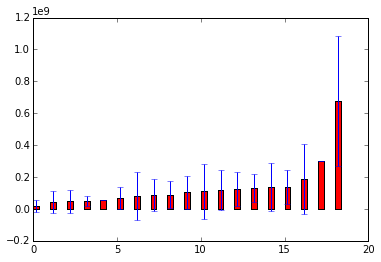
\includegraphics[max size={\textwidth}{\textheight}]{Data_Science_HW_1_files/Data_Science_HW_1_44_0.png}
    \par
    \end{center}
    
            \end{InvisibleVerbatim}
            
                \begin{InvisibleVerbatim}
                \vspace{-0.5\baselineskip}
\begin{alltt}(17316549.191666666, 37275316.941022627, '')
(43080325.745454542, 69492664.562573552, 'Based on Play')
(48227874.596774191, 72027608.622798443, 'Based on Real Life Events')
(50976952.666666664, 31039082.943294588, 'Compilation')
(56042592.0, 0.0, 'Musical Group Movie')
(67829046.375, 69669160.25334534, 'Based on Short Film')
(82096075.624755695, 151394921.57937899, 'Original Screenplay')
(85806723.833333328, 100582875.97222812, 'Based on Factual
Book/Article')
(90323299.0, 85497363.138208807, 'Based on Game')
(105214068.5, 102893984.07240242, 'Based on Magazine Article')
(110160386.52286585, 174017569.10990757, 'Based on Book/Short Story')
(120895934.69047619, 125194665.57854071, 'Remake')
(126238459.125, 107093456.7304098, 'Spin-Off')
(129627358.77777778, 88630856.183651105, 'Based on Musical/Opera')
(135444954.98113209, 149652925.57575357, 'Based on TV')
(139914559.625, 106264137.82101072, 'Traditional/Legend/Fairytale')
(188028113.21951219, 221622184.31693536, 'Based on Comic/Graphic
Novel')
(302469019.0, 0.0, 'Based on Toy')
(674664131.0, 408591074.13993609, 'Disney Ride')
\end{alltt}

            \end{InvisibleVerbatim}
            
        
    
Sigh.
        

        \renewcommand{\indexname}{Index}
        \printindex

    % End of document
    \end{document}


